\documentclass[11pt]{article}
\usepackage[margin=1in]{geometry}
\usepackage[T1]{fontenc}
\usepackage[utf8]{inputenc}
\usepackage{lmodern}
\usepackage{microtype}
\usepackage{amsmath,amssymb,mathtools}
\usepackage{amsthm}
\usepackage{booktabs}
\usepackage{graphicx}
\usepackage{xcolor}
\usepackage{hyperref}
\usepackage{enumitem}
\usepackage{tabularx}
\usepackage{float}
\usepackage{caption}
\usepackage{subcaption}

\hypersetup{
    colorlinks=true,
    linkcolor=blue!50!black,
    urlcolor=blue!60!black,
    citecolor=blue!50!black
}

% ── Notation shortcuts ──
\newcommand{\R}{\mathbb{R}}
\newcommand{\bx}{\mathbf{x}}
\newcommand{\bX}{\mathbf{X}}
\newcommand{\bz}{\mathbf{z}}
\newcommand{\bW}{\mathbf{W}}
\newcommand{\bb}{\mathbf{b}}
\newcommand{\bh}{\mathbf{h}}
\newcommand{\bs}{\mathbf{s}}
\newcommand{\bY}{\mathbf{Y}}
\newcommand{\bP}{\mathbf{P}}
\newcommand{\bH}{\mathbf{H}}
\newcommand{\bS}{\mathbf{S}}
\newcommand{\bZ}{\mathbf{Z}}
\newcommand{\bA}{\mathbf{A}}
\newcommand{\bone}{\mathbf{1}}
\newcommand{\bmu}{\boldsymbol{\mu}}
\newcommand{\bdelta}{\boldsymbol{\delta}}
\newtheorem{proposition}{Proposition}

\title{\textbf{From Linear Scores to a Single Hidden Layer:\\
A Mathematical Study of Simple Learning Systems}}
\author{Sharaf Feyzullayev \and Nicat Samadov \and Samir Abdullazade}
\date{\today}

\begin{document}
\maketitle

% ================================================================
%  ABSTRACT
% ================================================================
\begin{abstract}
This report investigates a mathematically precise question: when does a one-hidden-layer
neural network genuinely improve on a linear decision rule, and when is additional model
complexity unnecessary?  We compare Softmax Regression (a linear classifier) with a
single-hidden-layer neural network ($\tanh$ activation, hidden width $H{=}32$) on three tasks
of increasing geometric complexity---all implemented from scratch in NumPy with no
automatic-differentiation libraries.  On the \emph{Linear Gaussian} task, the Bayes-optimal
boundary is a hyperplane; both models achieve near-perfect accuracy, confirming that the
hidden layer provides no representational advantage when the data is linearly separable.
On the \emph{Moons} task, Softmax Regression fails because no hyperplane can separate two
interlocking arcs, while the neural network learns a curved boundary achieving near-$100\%$
accuracy.  On the \emph{Digits} benchmark ($d{=}64$, $K{=}10$), five-seed evaluation yields
$93.26\%\;\pm\;0.73\%$ for Softmax Regression versus $95.71\%\;\pm\;0.91\%$ for the neural
network---a modest but statistically robust gain.  A Track~A PCA/SVD analysis reveals that
20~principal components capture $89.6\%$ of variance and sustain $94.08\%$ Softmax accuracy,
exposing substantial linear structure in the input space.  A failure-case study with an
$H{=}2$ bottleneck ($58.97\%$ accuracy) demonstrates that representational capacity is a
prerequisite that optimisation cannot substitute.  Throughout, we derive the mathematics
rigorously, argue from evidence, and identify the boundaries of our conclusions.
\end{abstract}

% ================================================================
%  NOTATION TABLE
% ================================================================
\vspace{-0.3em}
\noindent\textbf{Notation.}\;
We adopt the following conventions throughout the report.
Lowercase bold ($\bx$) denotes column vectors; uppercase bold ($\bX$) denotes matrices.
A batch of $n$ inputs is stored row-wise in $\bX\in\R^{n\times d}$.
All symbols are defined before first use.
\begin{center}
\small
\begin{tabular}{@{}ll@{\qquad}ll@{}}
\toprule
$\bx\in\R^{d}$ & input feature vector &
$\bW_1\!\in\!\R^{d\times H}$ & hidden-layer weights \\
$y\in\{1,\dots,K\}$ & true class label &
$\bW_2\!\in\!\R^{H\times K}$ & output-layer weights \\
$K$ & number of classes &
$\bb_1\!\in\!\R^{H},\;\bb_2\!\in\!\R^{K}$ & bias vectors \\
$H$ & hidden-layer width &
$\bZ^{(1)},\bZ^{(2)}$ & pre-activation matrices \\
$n$ & batch/sample size &
$\bA^{(1)}$ & hidden activations \\
$d$ & input dimension &
$\hat{\bY}\!=\!\bP$ & predicted probability matrix \\
$\lambda$ & $L_2$ regularisation coefficient &
$\eta$ & learning rate \\
$\odot$ & Hadamard (element-wise) product &
$\|\cdot\|_F$ & Frobenius norm \\
\bottomrule
\end{tabular}
\end{center}

% ================================================================
\section{Introduction}
% ================================================================

The central question of this capstone is:
\begin{quote}
\itshape When does a one-hidden-layer nonlinear classifier genuinely improve on a linear
decision rule, and when is additional model complexity unnecessary?
\end{quote}

This question resists a blanket answer.  A responsible investigation requires
(i)~deriving the mathematics underlying each model class,
(ii)~constructing experiments whose geometry isolates the relevant differences,
(iii)~evaluating with repeated seeds and honest statistics, and
(iv)~acknowledging where conclusions do and do not extend.

We study two model classes, each producing a categorical distribution over $K$ classes:
\begin{enumerate}[label=(\roman*),leftmargin=2em,itemsep=0.15em]
  \item \textbf{Softmax Regression}---an affine map $\bz = \bW\bx + \bb$ followed by the
        softmax function.  The resulting decision boundary is a set of hyperplanes
        (affine surfaces in $\R^d$), so this model can only separate classes that are
        linearly distinguishable.
  \item \textbf{One-Hidden-Layer Neural Network}---a composition of an affine map, the
        $\tanh$ nonlinearity, and a second affine map followed by softmax.  The hidden layer
        performs a learned nonlinear coordinate change; the output layer then applies a linear
        classifier in the transformed space.  The resulting decision boundary can curve,
        and its complexity depends on the hidden width~$H$.
\end{enumerate}

Both models are evaluated on three tasks chosen to span a spectrum of geometric difficulty:
\begin{itemize}[leftmargin=1.4em,itemsep=0.15em]
  \item \textbf{Linear Gaussian}: two isotropic Gaussian blobs in $\R^2$---linearly separable
        by construction.
  \item \textbf{Moons}: two interleaving half-circles in $\R^2$---no hyperplane can separate
        them.
  \item \textbf{Digits}: an $8{\times}8$ handwritten-digit dataset ($d{=}64$, $K{=}10$) with a
        fixed train/validation/test split, representing a real-world task of moderate complexity.
\end{itemize}

Every model and optimiser is implemented from scratch in NumPy; no automatic-differentiation
libraries or high-level ML frameworks are used.  This design choice ensures that every gradient
computation is understood at the level of the chain rule, not hidden behind a library call.

% ================================================================
\section{Background and Mathematical Setup}
\label{sec:background}
% ================================================================

\subsection{Softmax Function and the Categorical Model}

For an input $\bx\in\R^d$, Softmax Regression computes logits $\bz = \bW\bx + \bb$, where
$\bW\in\R^{K\times d}$ and $\bb\in\R^K$.  These raw scores are converted to a valid
probability distribution via the softmax function:
\begin{equation}\label{eq:softmax}
  \hat{y}_k \;=\; P(y{=}k\mid\bx;\bW,\bb)
  \;=\; \frac{\exp(z_k)}{\displaystyle\sum_{j=1}^{K}\exp(z_j)},
  \qquad k=1,\dots,K.
\end{equation}
Two properties make this a well-defined categorical distribution:
(a)~each $\hat{y}_k > 0$ because the exponential is strictly positive, and
(b)~$\sum_k \hat{y}_k = 1$ by construction.
The logits $z_k$ therefore serve as unnormalised log-probabilities, and softmax is the
normalising map that converts them into a proper distribution over the $K$ classes.

\paragraph{Numerical stability.}
In practice, computing $\exp(z_k)$ directly risks overflow when logits are large.
The standard remedy exploits the shift-invariance of softmax:
$\mathrm{softmax}(\bz) = \mathrm{softmax}(\bz - c\bone)$ for any scalar $c$.
Choosing $c = \max_k z_k$ keeps all exponents non-positive, preventing overflow
while preserving exact arithmetic.

% ──────────────────────────────────────────────────────────────────
\subsection{Cross-Entropy Loss as Negative Log-Likelihood}
\label{sec:nll}

\paragraph{The probabilistic viewpoint.}
Given $N$ independent training pairs $\{(\bx^{(i)},y^{(i)})\}_{i=1}^{N}$, we model
each observed label $y^{(i)}$ as a draw from the categorical distribution parameterised
by the model.  The likelihood of the observed data under parameters $\theta=(\bW,\bb)$ is
\begin{equation}\label{eq:likelihood}
  \mathcal{L}(\theta)
  \;=\;\prod_{i=1}^{N} P\!\bigl(y^{(i)}\mid\bx^{(i)};\theta\bigr)
  \;=\;\prod_{i=1}^{N} \hat{y}_{y^{(i)}}^{(i)}.
\end{equation}

\paragraph{Step 1: Log-likelihood.}
Taking the natural logarithm converts the product into a sum, which is both numerically
stable and analytically convenient:
\begin{equation}\label{eq:loglik}
  \log\mathcal{L}(\theta)
  \;=\;\sum_{i=1}^{N} \log \hat{y}_{y^{(i)}}^{(i)}.
\end{equation}

\paragraph{Step 2: One-hot encoding.}
Introduce the one-hot vector $\mathbf{e}^{(i)}\in\{0,1\}^K$ with $e^{(i)}_k = 1$ if and
only if $k = y^{(i)}$.  Then $\log \hat{y}_{y^{(i)}}^{(i)} = \sum_{k=1}^{K} e^{(i)}_k
\log \hat{y}^{(i)}_k$, since only the true-class term survives.

\paragraph{Step 3: Negation and averaging.}
Negating the log-likelihood and dividing by $N$ yields the cross-entropy loss:
\begin{equation}\label{eq:ce}
  J(\theta) \;=\; -\,\frac{1}{N}\sum_{i=1}^{N}\sum_{k=1}^{K}
  e_k^{(i)}\log\hat{y}_k^{(i)}.
\end{equation}

\begin{proposition}
Minimising the cross-entropy loss~\eqref{eq:ce} is algebraically identical to maximising
the log-likelihood~\eqref{eq:loglik} of the observed labels under the categorical
model~\eqref{eq:softmax}.
\end{proposition}

This is not a heuristic design choice: cross-entropy is the principled loss function that
arises directly from treating classification as probabilistic inference under the
categorical likelihood.  Any other loss (e.g.\ squared error on probabilities) would be
mismatched to the generative assumption.

\paragraph{Connection to regularisation.}
Adding an $L_2$ penalty $\frac{\lambda}{2}\|\bW\|_F^2$ to $J$ is equivalent to placing an
isotropic Gaussian prior $\bW\sim\mathcal{N}(\mathbf{0},\lambda^{-1}\mathbf{I})$ on the
weights and performing maximum-a-posteriori (MAP) estimation instead of pure MLE.
We use $\lambda=10^{-4}$ throughout to gently discourage large weights without dominating
the learning signal.

% ──────────────────────────────────────────────────────────────────
\subsection{Conceptual Overview of Backpropagation}
\label{sec:backprop-concept}

Before writing any gradient formulas, it is essential to understand what backpropagation
\emph{does} rather than just \emph{how} it computes.

A neural network is a composition of parameterised functions.  In the forward pass, data
flows through a sequence of transformations---affine projections, element-wise
nonlinearities, softmax---producing intermediate quantities (pre-activations, hidden
activations, logits, probabilities) and ultimately a scalar loss~$J$.  Each of these
intermediate quantities is saved for later use.

Backpropagation is the systematic, reverse-order application of the multivariate chain rule
through this computation graph.  Starting from the scalar loss at the output, we compute how
$J$ changes with respect to the final layer's inputs.  We then step backward, one layer at a
time: at each stage, the incoming ``error signal'' (the gradient from the layer above) is
multiplied by the local Jacobian of the current transformation.  This factorisation
decomposes the global sensitivity into \emph{localised} directional information for every
parameter.

Concretely, backpropagation answers the question:
\begin{quote}
\itshape If the loss increased by a small amount, which parameters are responsible, in which
direction, and by how much?
\end{quote}

Three properties make backpropagation practical:
\begin{enumerate}[leftmargin=2em,itemsep=0.15em]
  \item \textbf{Locality.}  Each layer only needs its own inputs, outputs, and the upstream
        gradient---never the full computation graph.
  \item \textbf{Efficiency.}  The cost of one backward pass is proportional to one forward
        pass (roughly $2{\times}$ total), regardless of the number of parameters.
  \item \textbf{Exactness.}  No finite-difference approximations are involved; the gradients
        are analytically exact up to floating-point arithmetic.
\end{enumerate}

% ──────────────────────────────────────────────────────────────────
\subsection{Complete Gradient Derivation for the One-Hidden-Layer Network}
\label{sec:gradient-derivation}

We now derive every parameter gradient in closed form.  Consider a minibatch
$\bX\in\R^{n\times d}$ with one-hot label matrix $\bY\in\{0,1\}^{n\times K}$.

\paragraph{Forward pass (four stages).}
\begin{align}
  \bZ^{(1)} &= \bX\,\bW_1 + \bone\,\bb_1^\top
    & &\in\R^{n\times H}, \label{eq:fwd1}\\
  \bA^{(1)} &= \tanh\!\bigl(\bZ^{(1)}\bigr)
    & &\in\R^{n\times H}, \label{eq:fwd2}\\
  \bZ^{(2)} &= \bA^{(1)}\bW_2 + \bone\,\bb_2^\top
    & &\in\R^{n\times K}, \label{eq:fwd3}\\
  \hat{\bY}  &= \mathrm{softmax}_{\text{row}}\!\bigl(\bZ^{(2)}\bigr)
    & &\in\R^{n\times K}. \label{eq:fwd4}
\end{align}
Here $\bone\in\R^n$ is the all-ones vector, used to broadcast bias vectors across the batch.
Equation~\eqref{eq:fwd1} projects inputs into the hidden space; \eqref{eq:fwd2} applies the
nonlinearity element-wise; \eqref{eq:fwd3} maps hidden activations to class logits;
\eqref{eq:fwd4} normalises logits into probabilities.

\paragraph{Loss.}
The average cross-entropy over the minibatch:
\begin{equation}\label{eq:batch-ce}
  J = -\frac{1}{n}\sum_{i=1}^{n}\sum_{k=1}^{K} Y_{ik}\log\hat{Y}_{ik}.
\end{equation}

\paragraph{Step 1: Output-layer error signal.}
A key result from the calculus of softmax combined with cross-entropy gives the gradient
with respect to the pre-softmax logits:
\begin{equation}\label{eq:delta2}
  \bdelta^{(2)}
  \;=\;\frac{\partial J}{\partial \bZ^{(2)}}
  \;=\;\frac{1}{n}\bigl(\hat{\bY}-\bY\bigr)
  \quad\in\R^{n\times K}.
\end{equation}

\textit{Derivation.}  For a single sample $i$ and class $k$, the softmax Jacobian gives
$\frac{\partial \hat{Y}_{ij}}{\partial Z^{(2)}_{ik}} = \hat{Y}_{ij}(\delta_{jk} - \hat{Y}_{ik})$,
where $\delta_{jk}$ is the Kronecker delta.  Therefore:
\[
  \frac{\partial J}{\partial Z^{(2)}_{ik}}
  = -\frac{1}{n}\sum_{j=1}^{K} Y_{ij}\,
    \frac{1}{\hat{Y}_{ij}}\,\hat{Y}_{ij}(\delta_{jk} - \hat{Y}_{ik})
  = -\frac{1}{n}\Bigl(\underbrace{\sum_j Y_{ij}}_{=\,1}\,\delta_{jk}
    - \hat{Y}_{ik}\underbrace{\sum_j Y_{ij}}_{=\,1}\Bigr)_{j=k}
  = \frac{1}{n}(\hat{Y}_{ik} - Y_{ik}).
\]
The simplification follows because $\bY$ is one-hot, so $\sum_j Y_{ij} = 1$.

\paragraph{Step 2: Output-layer parameter gradients.}
Since $\bZ^{(2)} = \bA^{(1)}\bW_2 + \bone\bb_2^\top$, the chain rule gives:
\begin{align}
  \frac{\partial J}{\partial \bW_2}
  &= \bigl(\bA^{(1)}\bigr)^\top \bdelta^{(2)}
  \;\in\;\R^{H\times K},
  \label{eq:gW2}\\[4pt]
  \frac{\partial J}{\partial \bb_2}
  &= \bigl(\bdelta^{(2)}\bigr)^\top\bone
  \;\in\;\R^{K}.
  \label{eq:gb2}
\end{align}
Equation~\eqref{eq:gW2} is a matrix product that sums, over all samples, the outer product
of each hidden activation vector with its error signal.  Equation~\eqref{eq:gb2} sums the
error across samples.

\paragraph{Step 3: Hidden-layer error (backpropagation through $\tanh$).}
The error signal is transported backward through $\bW_2$ and modulated by the local
$\tanh$ derivative.  Since $\tanh'(z) = 1 - \tanh^2(z)$:
\begin{equation}\label{eq:delta1}
  \bdelta^{(1)}
  \;=\;
  \bigl(\bdelta^{(2)}\,\bW_2^\top\bigr)
  \;\odot\;
  \bigl(1 - \bA^{(1)}\odot\bA^{(1)}\bigr)
  \quad\in\R^{n\times H}.
\end{equation}
The first factor $\bdelta^{(2)}\bW_2^\top$ propagates the output error across the linear map;
the Hadamard product with $(1 - \bA^{(1)}\odot\bA^{(1)})$ scales each component by the
local responsiveness of the $\tanh$ activation at that point.  Where the activation is
saturated ($|\tanh(z)|\approx 1$), the derivative is near zero, attenuating the gradient.

\paragraph{Step 4: Hidden-layer parameter gradients.}
Since $\bZ^{(1)} = \bX\bW_1 + \bone\bb_1^\top$:
\begin{align}
  \frac{\partial J}{\partial \bW_1}
  &= \bX^\top\,\bdelta^{(1)}
  \;\in\;\R^{d\times H},
  \label{eq:gW1}\\[4pt]
  \frac{\partial J}{\partial \bb_1}
  &= \bigl(\bdelta^{(1)}\bigr)^\top\bone
  \;\in\;\R^{H}.
  \label{eq:gb1}
\end{align}

These four steps constitute the complete backpropagation for our architecture.
With $L_2$ regularisation, we add $\lambda\bW_\ell$ to the weight gradient at each
layer~$\ell$, corresponding to the prior term in MAP estimation.

\paragraph{Parameter count.}  Softmax Regression has $Kd + K$ parameters.
The neural network has $(dH + H) + (HK + K) = H(d+K) + H + K$ parameters.
For our Digits configuration ($d{=}64$, $H{=}32$, $K{=}10$), this yields
$64\times 32 + 32 + 32\times 10 + 10 = 2{,}410$ parameters versus $64\times 10 + 10 = 650$
for Softmax Regression---roughly $3.7{\times}$ more.

% ──────────────────────────────────────────────────────────────────
\subsection{Geometric Compatibility: Gaussian vs.\ Moons}
\label{sec:geometry}

\paragraph{Why the Gaussian task is well matched to a linear decision rule.}
The Linear Gaussian dataset consists of two classes drawn from $\mathcal{N}(\bmu_0,\sigma^2\mathbf{I})$
and $\mathcal{N}(\bmu_1,\sigma^2\mathbf{I})$ with equal priors.  By Bayes' theorem, the
log-posterior ratio is:
\begin{equation}\label{eq:logodds}
  \log\frac{P(y{=}1\mid\bx)}{P(y{=}0\mid\bx)}
  \;=\;
  \frac{1}{\sigma^2}(\bmu_1-\bmu_0)^\top\bx
  \;-\;\frac{1}{2\sigma^2}\bigl(\|\bmu_1\|^2-\|\bmu_0\|^2\bigr).
\end{equation}
This is an \emph{affine} function of $\bx$: the Bayes-optimal decision boundary
$\{P(y{=}1\mid\bx)=0.5\}$ is a hyperplane whose normal direction is $\bmu_1-\bmu_0$.
Since Softmax Regression parameterises exactly the family of affine classifiers, it can
represent the optimal boundary.  A hidden layer adds parameters but cannot change the
boundary geometry in any meaningful way---it merely over-parameterises a function that is
already in the linear model's hypothesis class.

\paragraph{Why the Moons task requires nonlinearity.}
The Moons dataset arranges two classes as interleaving half-circles.  Consider the upper arc
(class~0) centred at the origin and the lower arc (class~1) offset and flipped.  Any
separating hyperplane in $\R^2$ is a straight line, but the two arcs curve into each other's
coordinate half-space---no single line can avoid cutting through both classes.  Formally, the
classes are \emph{not linearly separable}: there exist no $\bW,\bb$ such that
$\mathrm{sign}(\bW\bx+\bb)$ correctly classifies all points.

The hidden layer addresses this by applying the map
$\bh = \tanh(\bW_1\bx + \bb_1) \in \R^H$.  This is a learned nonlinear coordinate
transformation.  In the new $H$-dimensional space, the previously entangled arcs can become
linearly separable---the second affine map $\bW_2\bh + \bb_2$ then draws a hyperplane in the
\emph{transformed} coordinates.  The network's power lies not in the final linear
classifier but in the representation it creates beforehand.

% ================================================================
\section{Methods}
\label{sec:methods}
% ================================================================

\paragraph{Datasets.}
Three datasets, all loaded from the starter pack with no additional preprocessing:
\begin{enumerate}[label=\arabic*.,leftmargin=2em,itemsep=0.15em]
  \item \textbf{Linear Gaussian}: 400 points in $\R^2$, two isotropic Gaussian blobs
        with mild overlap.
  \item \textbf{Moons}: 400 points in $\R^2$, two interlocking half-circles with
        added noise.
  \item \textbf{Digits}: $d{=}64$ pixel features from the UCI handwritten digits dataset,
        with a fixed stratified split of 1\,258~train / 270~validation / 269~test samples
        across $K{=}10$ classes.  Features are pre-scaled to $[0,1]$.
\end{enumerate}

\paragraph{Implementation.}
Both models are implemented entirely in NumPy.  Softmax is computed with the row-wise
maximum subtraction for numerical stability.  Gradients follow the derivations in
Section~\ref{sec:gradient-derivation}.  Three optimisers---SGD, Momentum ($\mu{=}0.9$),
and Adam ($\beta_1{=}0.9$, $\beta_2{=}0.999$, $\varepsilon{=}10^{-8}$)---are implemented
from scratch.

\paragraph{Training protocol for the Digits benchmark.}
A strict protocol ensures fair comparison:
\begin{itemize}[leftmargin=1.4em,itemsep=0.15em]
  \item Mini-batch size: $64$.
  \item $L_2$ regularisation: $\lambda=10^{-4}$ for both models.
  \item Epoch budget: 200.
  \item Model selection: the checkpoint with the lowest \emph{validation} cross-entropy
        within the epoch budget is retained as the final model.
  \item Softmax baseline: mini-batch SGD, $\eta{=}0.05$.
  \item Neural network default: $H{=}32$, SGD, $\eta{=}0.05$.
\end{itemize}

\paragraph{Training protocol for synthetic tasks.}
Both models are trained with full-batch gradient descent (batch size equals training set
size) for 300~epochs.  Softmax Regression uses SGD ($\eta{=}0.1$); the neural network uses
Adam ($\eta{=}0.01$) to ensure it can fully explore the nonlinear feature space.
$L_2$ regularisation is set to $\lambda{=}10^{-5}$.  The best validation checkpoint is
reported.

\paragraph{Repeated-seed evaluation.}
On Digits, each final configuration is trained with five random seeds ($s \in \{0,1,2,3,4\}$).
For each seed, the test set is evaluated \emph{exactly once} after validation-based model
selection.  We report mean and $95\%$ confidence interval:
\begin{equation}\label{eq:ci}
  \bar{x}\;\pm\;t_{0.025,\,4}\cdot\frac{s}{\sqrt{5}}
  \;=\;\bar{x}\;\pm\;2.776\cdot\frac{s}{\sqrt{5}},
\end{equation}
where $s$ is the sample standard deviation and $t_{0.025,4}$ is the critical value of the
$t$-distribution with 4 degrees of freedom at the $2.5\%$ tail.

% ================================================================
\section{Implementation Sanity Checks}
\label{sec:sanity}
% ================================================================

Before running any experiment, five automated checks verified fundamental correctness:

\begin{enumerate}[label=\textbf{Check~\arabic*.},leftmargin=3em,itemsep=0.3em]
  \item \textbf{Probability normalisation.}
        On three test logit vectors---including the numerically extreme case
        $\bz=[-100,\;0,\;100]$---the \texttt{stable\_softmax} function returns rows that
        sum to $1.0$ to machine precision.  This confirms that the max-subtraction
        stabilisation is correctly implemented.
        \hfill$\checkmark$\;PASS

  \item \textbf{Monotonic loss decrease.}
        A fresh Softmax Regression model was updated for 50~SGD steps on a 10-sample
        batch ($d{=}2$, $K{=}2$, $\eta{=}0.5$, no regularisation).  The loss decreased
        monotonically from $0.7260$ to $0.1563$, confirming that the gradient direction
        is correct and the step size is reasonable.
        \hfill$\checkmark$\;PASS

  \item \textbf{Numerical gradient verification.}
        For each parameter matrix ($\bW_1, \bW_2, \bb_1, \bb_2$) of a small neural
        network ($d{=}2$, $H{=}4$, $K{=}2$), the analytical gradient from backpropagation
        was compared against a centred finite-difference approximation
        ($\varepsilon{=}10^{-5}$).  The maximum absolute discrepancy was below $10^{-4}$
        for all parameters, confirming that the chain-rule implementation is correct.
        \hfill$\checkmark$\;PASS

  \item \textbf{No NaN/Inf in parameters.}
        After 20~epochs of training a neural network ($H{=}8$) on a tiny dataset, all
        parameter arrays were verified to contain no NaN or Inf values.
        \hfill$\checkmark$\;PASS

  \item \textbf{Overfitting a micro-dataset.}
        A neural network ($H{=}16$) was trained on 10 hand-chosen samples for 200~Adam
        steps.  The final training accuracy reached $100\%$, confirming that the forward
        and backward passes are mutually consistent and the model has sufficient capacity
        to memorise a small dataset.
        \hfill$\checkmark$\;PASS
\end{enumerate}

All five checks pass automatically.  No NaN or Inf values were encountered during any
experiment reported in this paper.

% ================================================================
\section{Experiments}
\label{sec:experiments}
% ================================================================

\subsection{Synthetic Decision Boundaries}

\paragraph{Linear Gaussian.}
Figure~\ref{fig:comparison_gaussian} shows that both models learn essentially the same
straight boundary.  The neural network produces slightly different probability contours
(reflecting the $\tanh$ nonlinearity), but the 50\%-probability line---the actual decision
boundary---is in the same location as the Softmax Regression boundary.  Both achieve
near-perfect accuracy.

This confirms the geometric argument of Section~\ref{sec:geometry}: when the Bayes-optimal
boundary is a hyperplane, the hidden layer provides no representational advantage.  The
additional $H(d+K)+H$ parameters of the neural network are wasted---they merely reparameterise
a function already representable by the simpler model.

\begin{figure}[H]
  \centering
  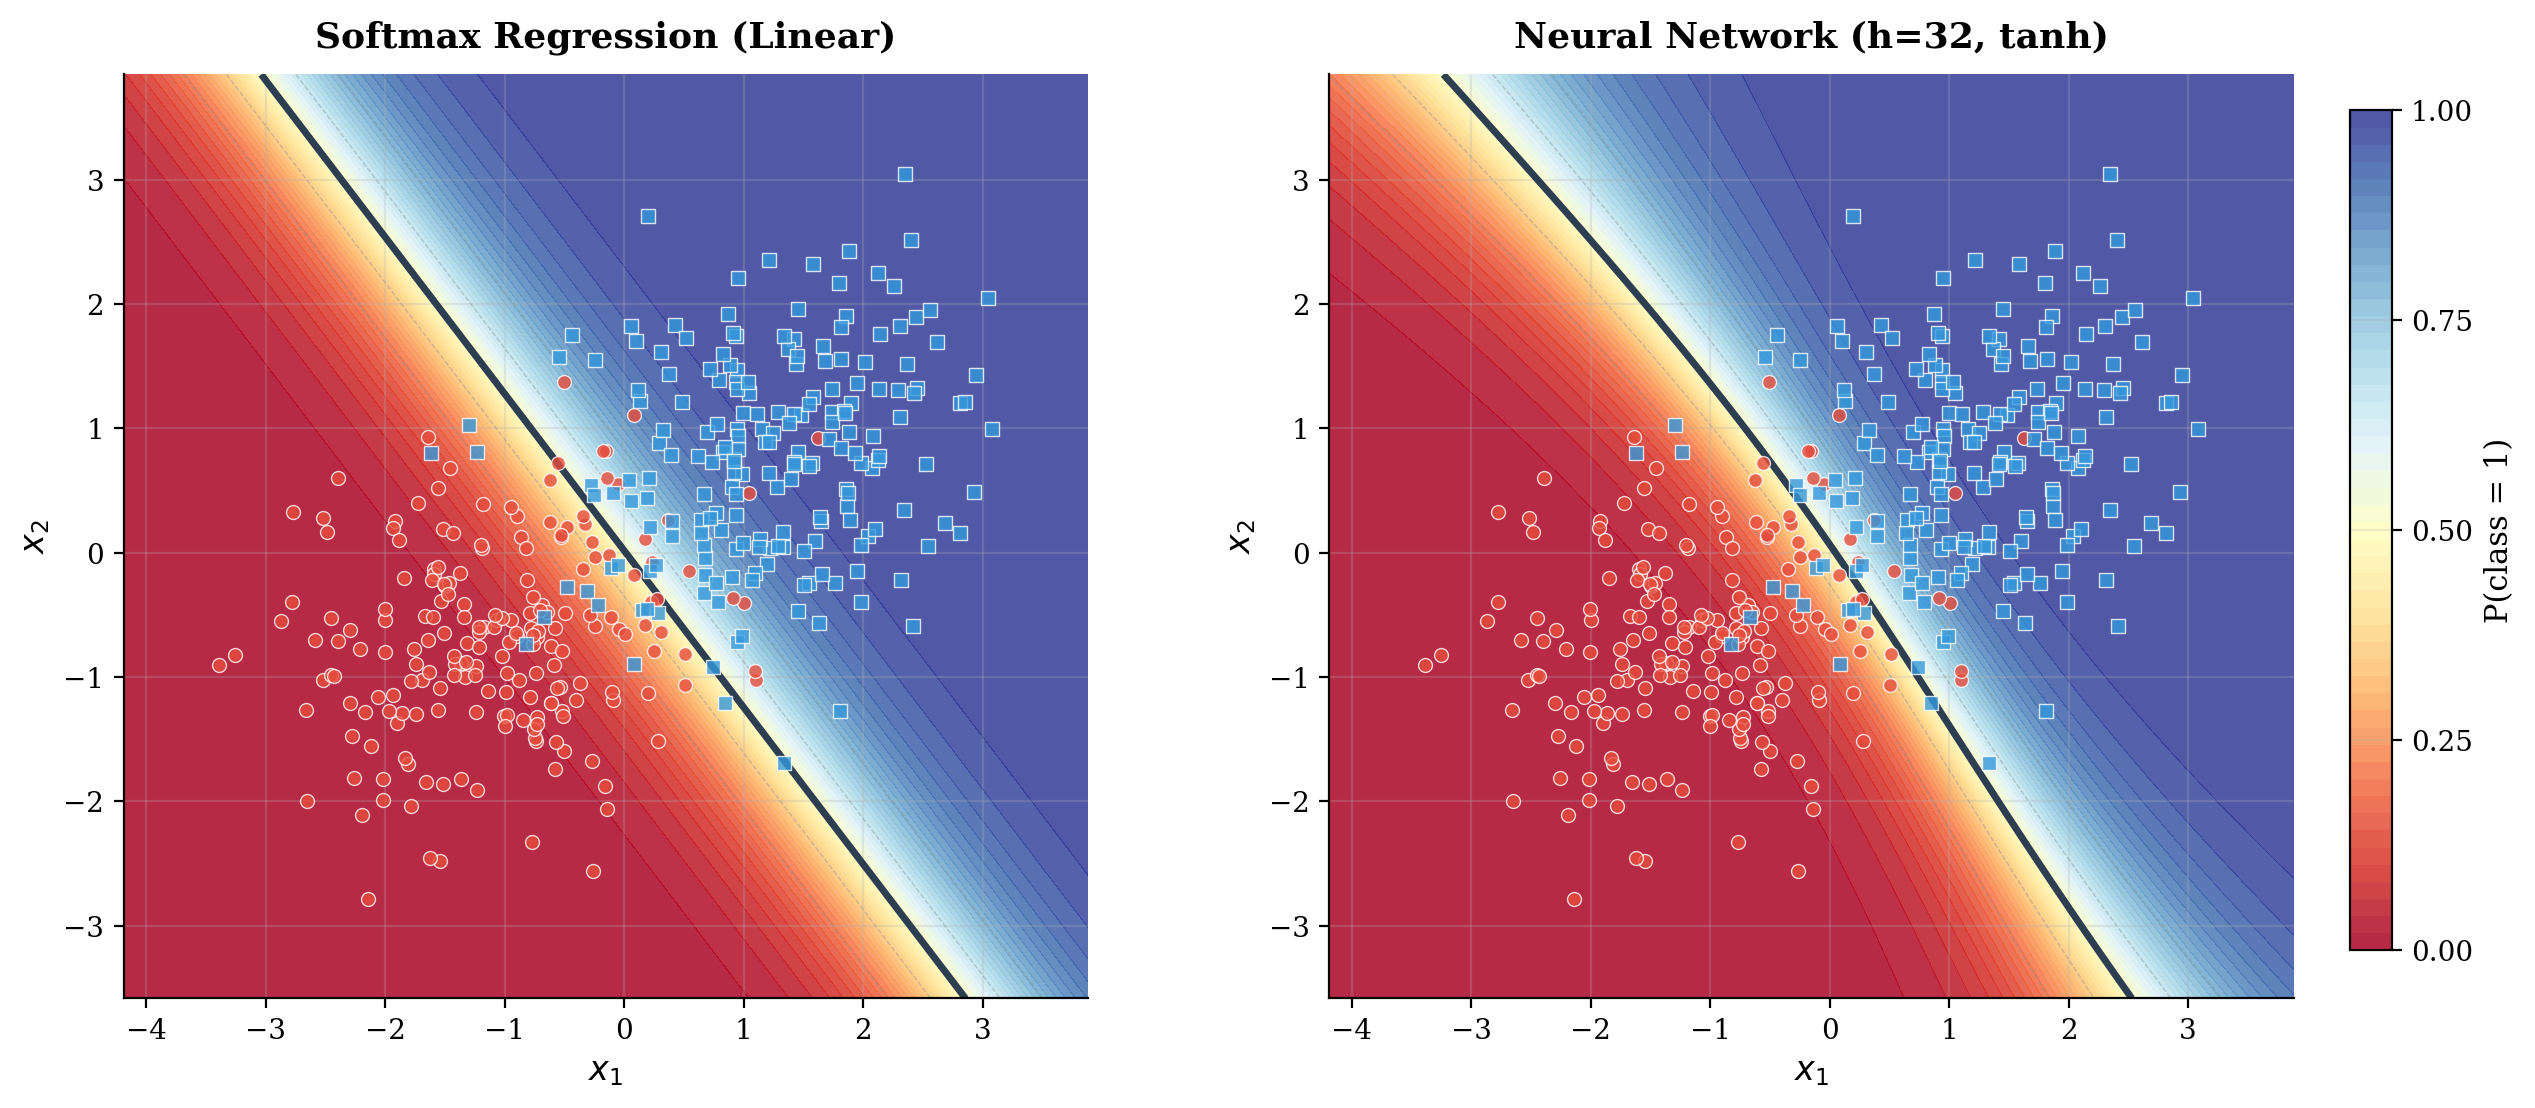
\includegraphics[width=\textwidth]{../figures/comparison_lineargaussian.png}
  \caption{Decision boundaries on the Linear Gaussian task.  Left: Softmax Regression.
           Right: Neural Network ($H{=}32$).  Both produce a near-identical linear
           separator, confirming that the hidden layer adds no geometric value when
           the optimal boundary is already a hyperplane.}
  \label{fig:comparison_gaussian}
\end{figure}

\paragraph{Moons.}
Figure~\ref{fig:comparison_moons} reveals the fundamental geometric difference between the
two model classes.  Softmax Regression is constrained to place a straight line through
the curved data, resulting in substantial misclassification along the interleaving arcs.
The neural network ($H{=}32$), by contrast, learns a smooth, curved boundary that wraps
around the two half-circles and achieves near-$100\%$ accuracy.

The mechanism is the one described in Section~\ref{sec:geometry}: the hidden layer maps the
original 2-D coordinates into a 32-dimensional space via $\tanh(\bW_1\bx+\bb_1)$, where
the previously entangled arcs become linearly separable.  The output layer then draws a
hyperplane in this new space, which maps back to a \emph{curve} in the original $\R^2$.

\begin{figure}[H]
  \centering
  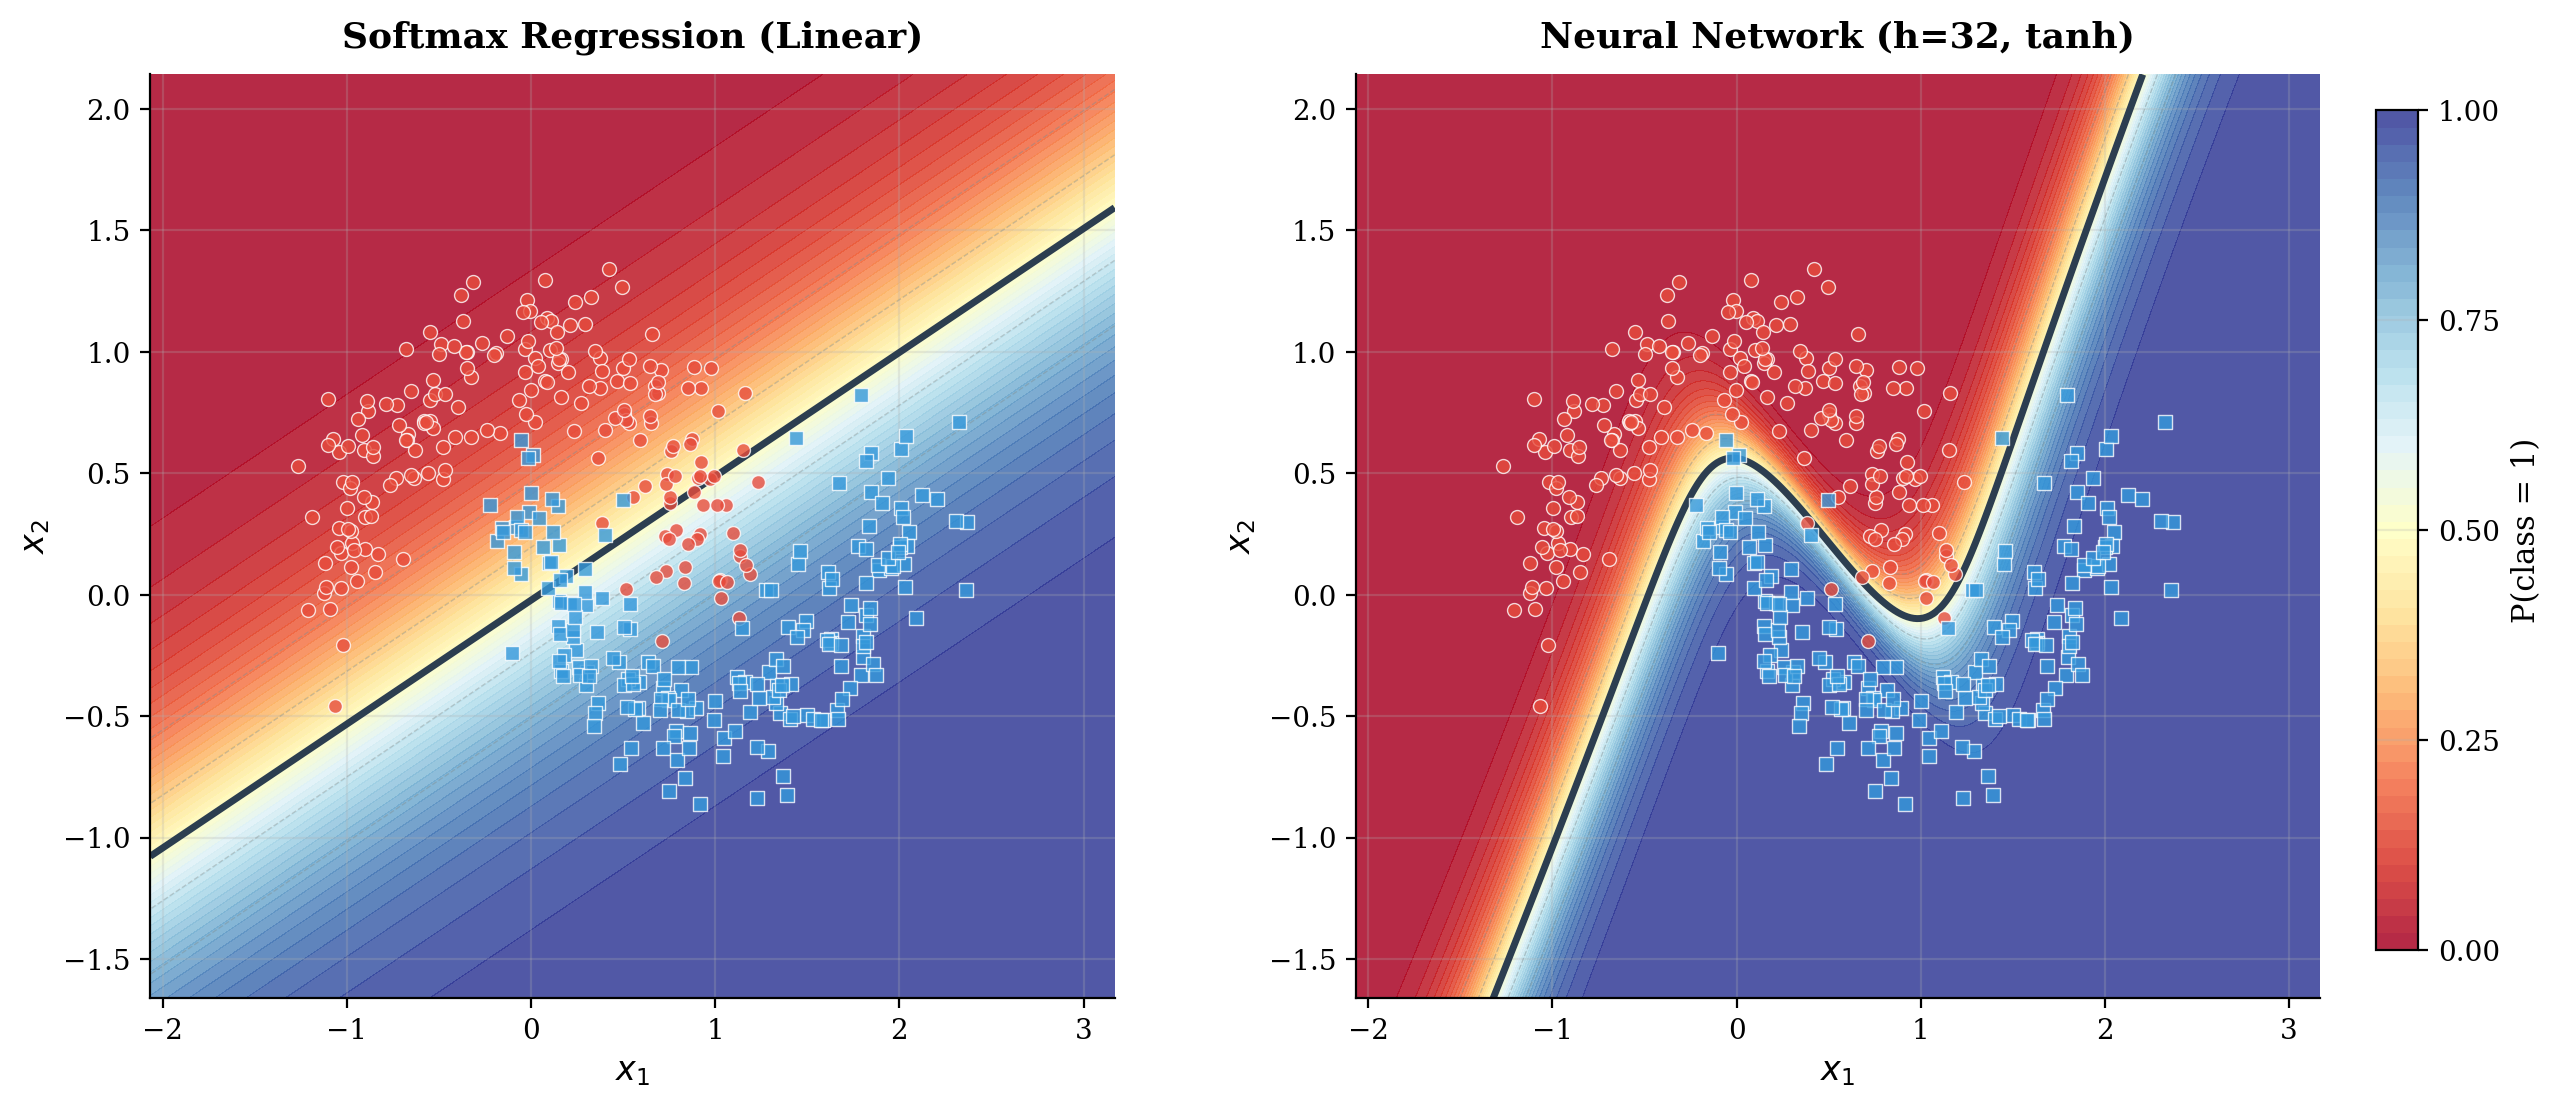
\includegraphics[width=\textwidth]{../figures/comparison_moons.png}
  \caption{Decision boundaries on the Moons task.  Left: Softmax Regression (linear,
           fails).  Right: Neural Network ($H{=}32$, succeeds).  The hidden layer
           transforms the input space so that the interlocking arcs become linearly
           separable.}
  \label{fig:comparison_moons}
\end{figure}

% ──────────────────────────────────────────────────────────────────
\subsection{Capacity Ablation on Moons}

To understand how hidden width affects the learned boundary, we trained the neural network
on Moons with $H\in\{2,8,32\}$ (Figure~\ref{fig:ablation}).

\begin{itemize}[leftmargin=1.4em,itemsep=0.15em]
  \item $H{=}2$: The model maps $\R^2\to\R^2$ via $\tanh$, so the transformation preserves
        dimensionality.  With only two hidden units, the model produces angular,
        low-confidence boundaries and cannot capture the full curvature of the arcs.
  \item $H{=}8$: The map $\R^2\to\R^8$ provides enough dimensions for a reasonable
        approximation to the curved boundary, though confidence near the boundary remains
        uneven.
  \item $H{=}32$: The map $\R^2\to\R^{32}$ provides ample room.  The boundary is smooth,
        high-confidence, and tightly hugs the data manifold.
\end{itemize}

This ablation demonstrates a monotonic relationship between hidden width and boundary quality
\emph{on this task}, because the intrinsic complexity of the Moons separation requires
nonlinear expressiveness that grows with $H$.  On the Gaussian task, by contrast, all three
widths produce essentially the same linear boundary, because the task's geometry does not
demand nonlinear features.

\begin{figure}[H]
  \centering
  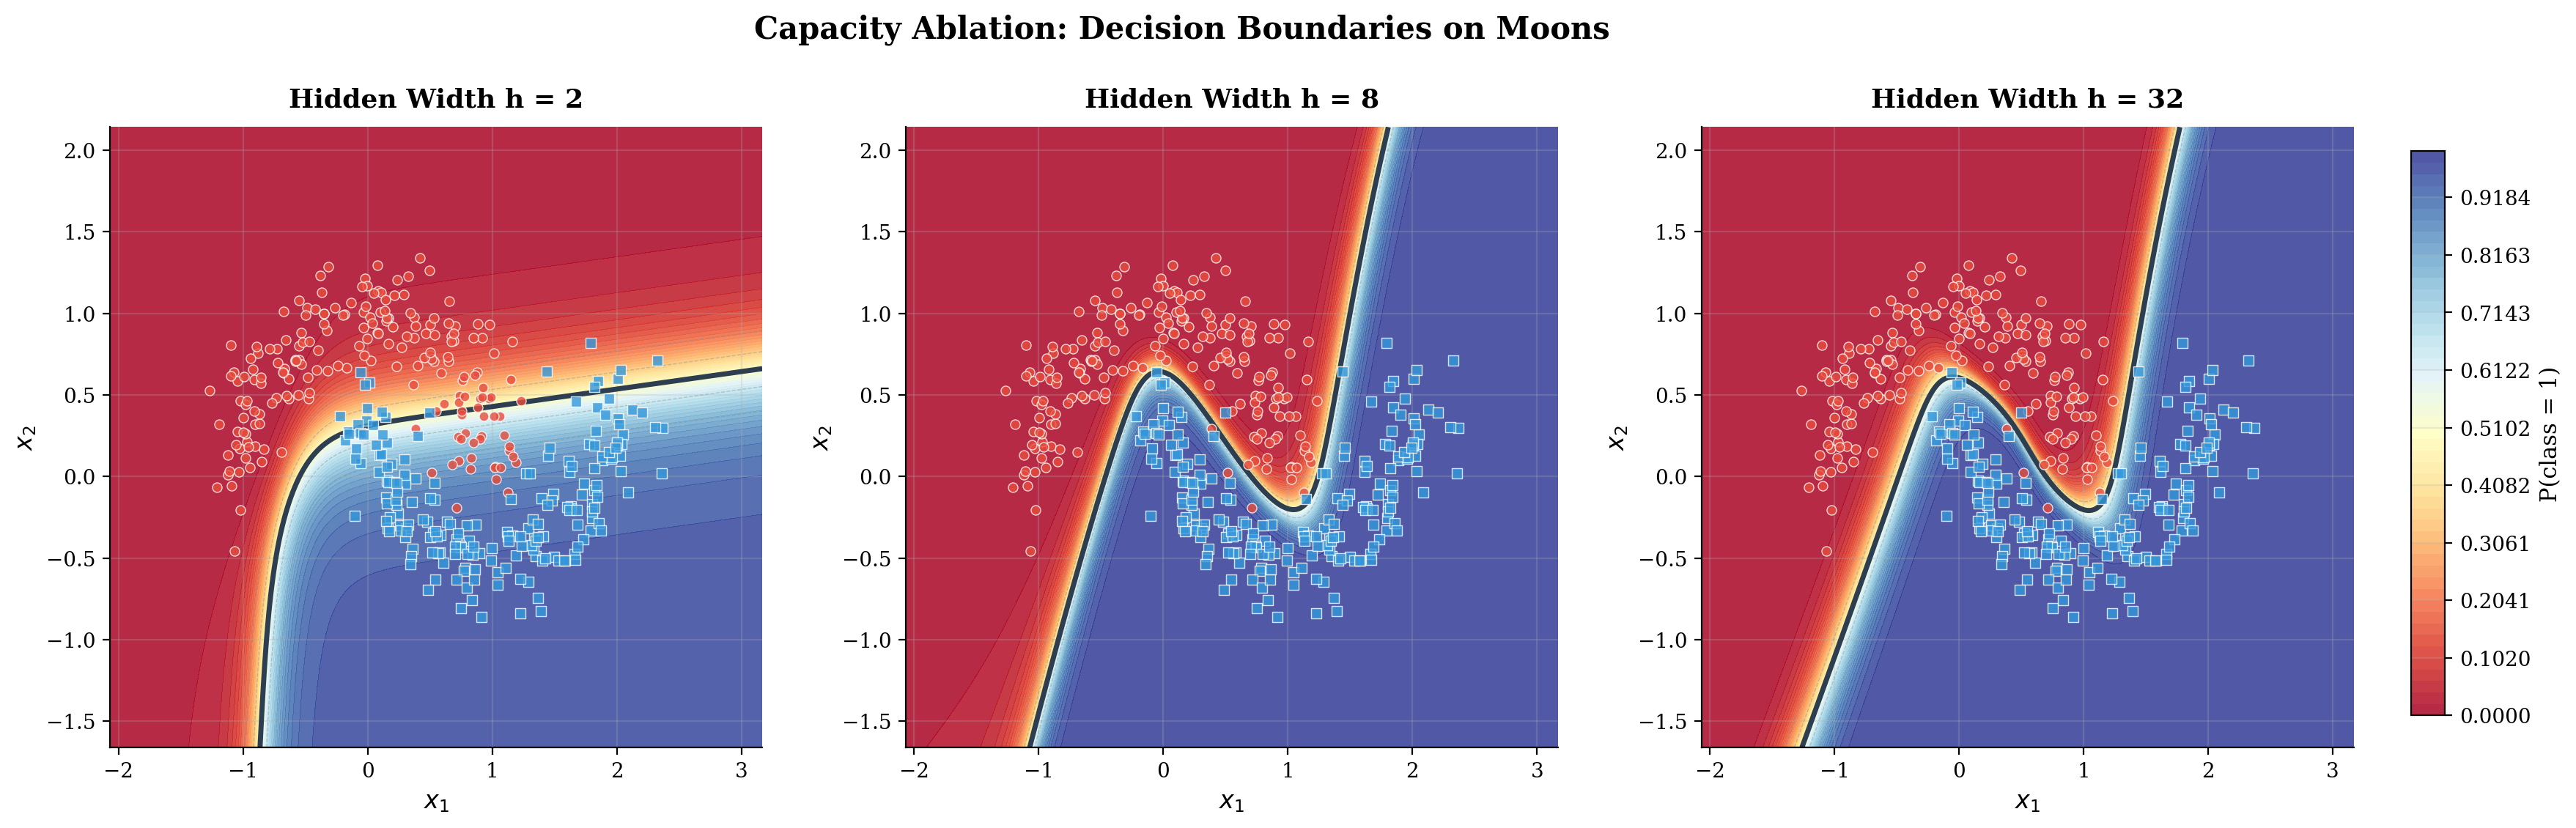
\includegraphics[width=\textwidth]{../figures/capacity_ablation_boundaries.png}
  \caption{Capacity ablation on Moons.  Left to right: $H{=}2$, $H{=}8$, $H{=}32$.
           Boundary smoothness and classification confidence increase with hidden width.}
  \label{fig:ablation}
\end{figure}

% ──────────────────────────────────────────────────────────────────
\subsection{Digits Benchmark}

Table~\ref{tab:digits_main} summarises the core Digits comparison using
validation-selected best checkpoints over 200~epochs and five-seed evaluation.

\begin{table}[H]
\centering
\caption{Digits benchmark: five-seed summary (mean $\pm$ 95\% CI).}
\label{tab:digits_main}
\begin{tabular}{@{}lcc@{}}
\toprule
\textbf{Model} & \textbf{Test Accuracy} & \textbf{Test Cross-Entropy} \\
\midrule
Softmax Regression & $93.26\%\;\pm\;0.73\%$ & $0.2692\;\pm\;0.0067$ \\
Neural Network ($H{=}32$) & $95.71\%\;\pm\;0.91\%$ & $0.1566\;\pm\;0.0162$ \\
\bottomrule
\end{tabular}
\end{table}

The neural network improves test accuracy by ${\sim}2.5$ percentage points and reduces
cross-entropy by ${\sim}42\%$.  The improvement is modest but statistically consistent:
the $95\%$ confidence intervals for the two models do not overlap.  The cross-entropy
reduction is proportionally larger than the accuracy gain, indicating that the neural
network produces better-calibrated probability estimates, not just more correct hard
predictions.

Figure~\ref{fig:loss_curves_digits} shows representative training and validation loss curves.
The neural network converges to a lower validation loss, and the gap between training and
validation loss is small for both models, indicating that neither suffers from severe
overfitting within the 200-epoch budget with $\lambda{=}10^{-4}$ regularisation.

\begin{figure}[H]
  \centering
  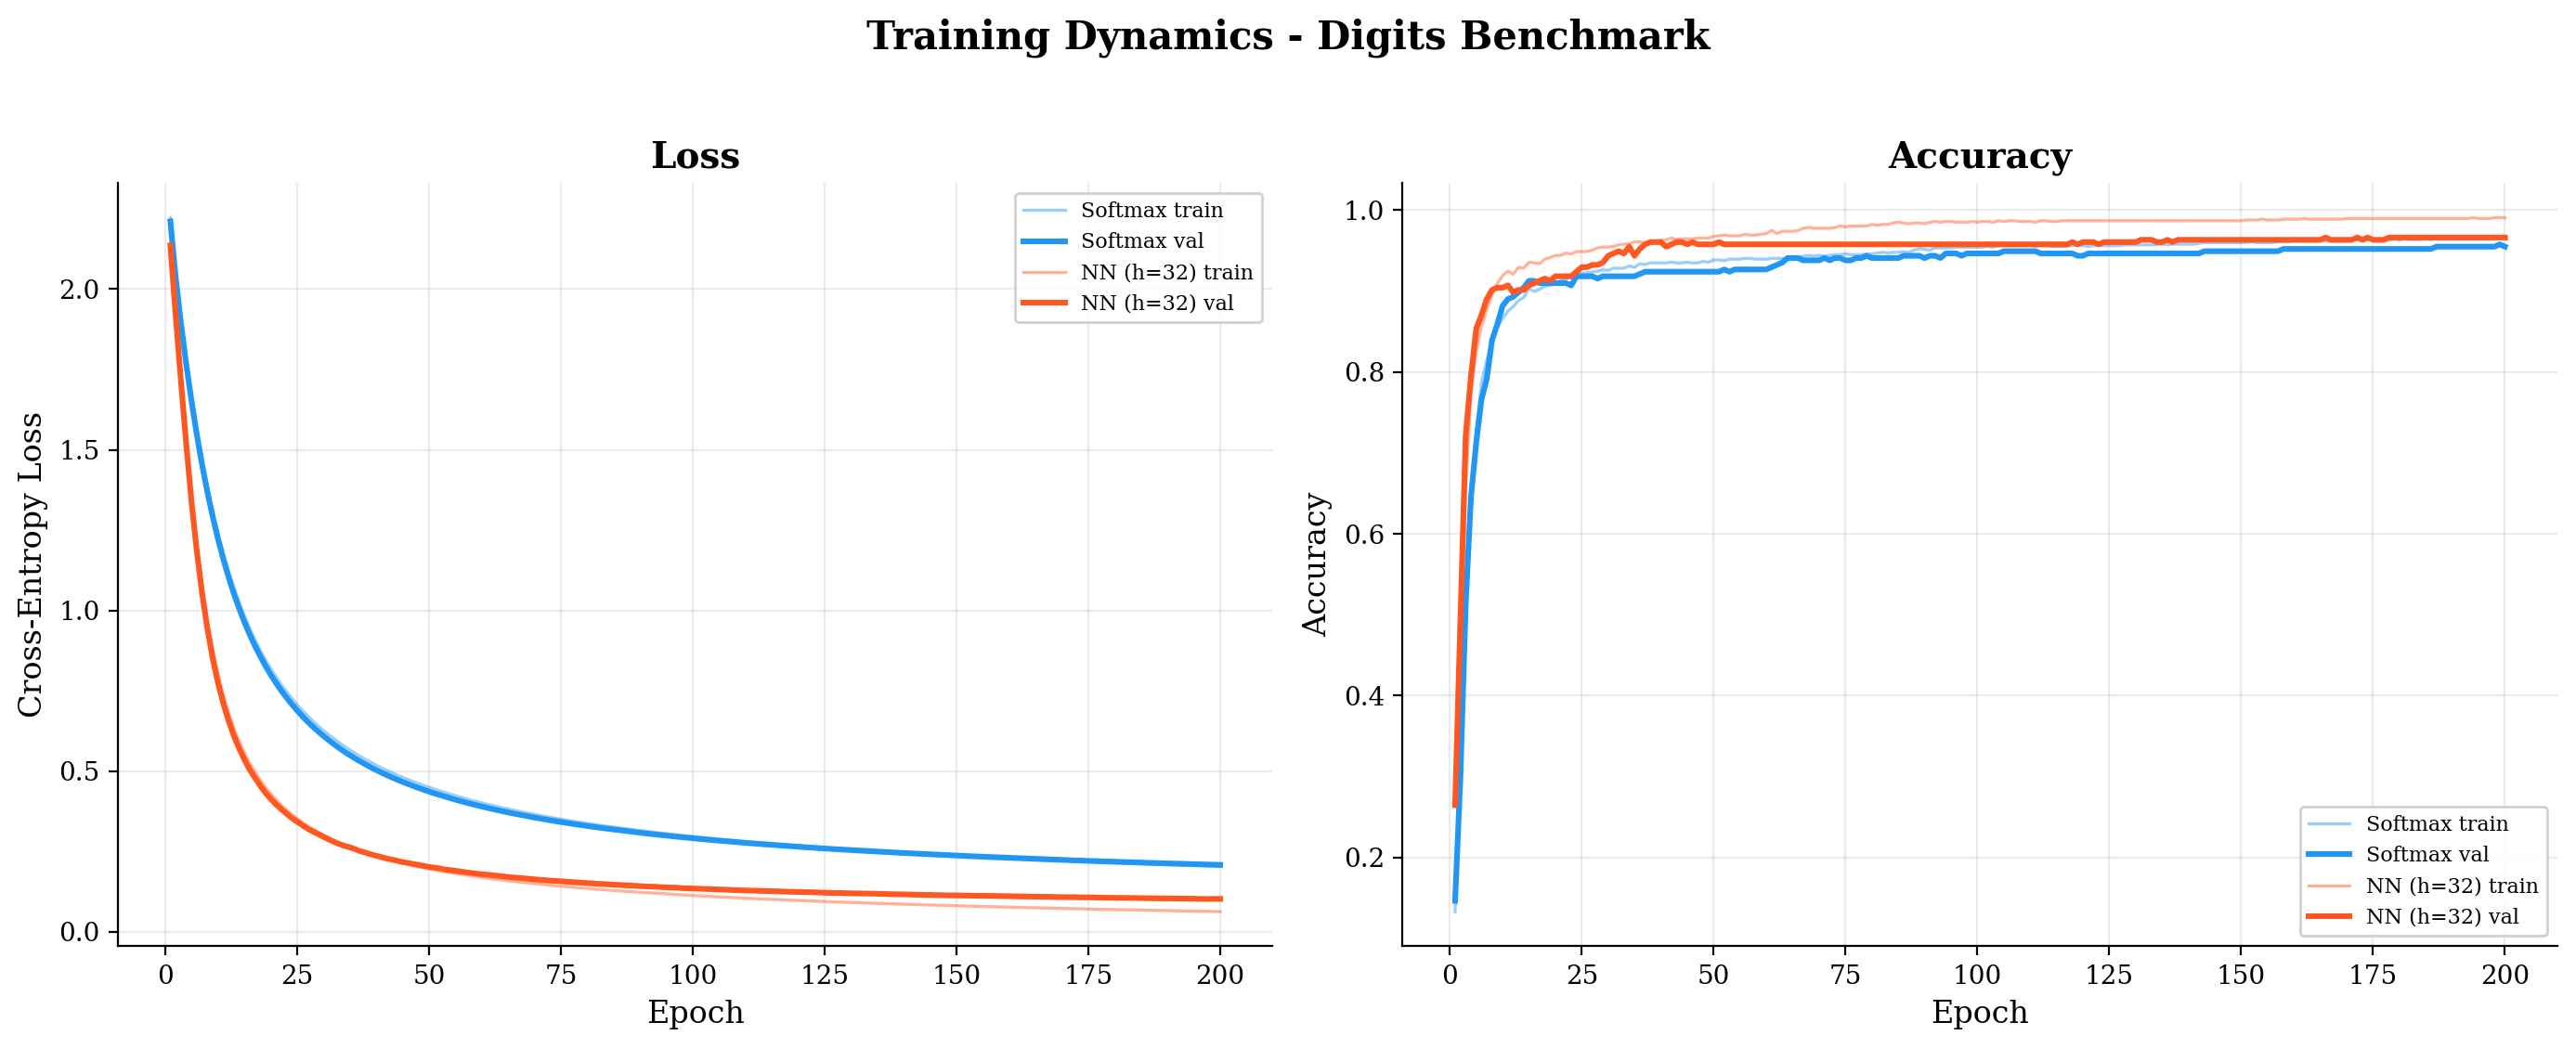
\includegraphics[width=\textwidth]{../figures/loss_curves_digits.png}
  \caption{Training dynamics on the Digits benchmark (single representative seed).
           The neural network reaches a lower validation loss and shows no severe
           train--val gap.}
  \label{fig:loss_curves_digits}
\end{figure}

% ──────────────────────────────────────────────────────────────────
\subsection{Optimizer Study on Digits}
\label{sec:optimizer}

Three optimisers were compared on the neural network ($H{=}32$) using fixed hyperparameters
from the Digits protocol.  The Softmax Regression baseline is \emph{not} part of this
comparison; it uses SGD throughout.

\begin{table}[H]
\centering
\caption{Optimizer study on Digits (NN, $H{=}32$, best validation checkpoint).}
\label{tab:optimizers}
\begin{tabular}{@{}lccc@{}}
\toprule
\textbf{Optimizer} & \textbf{Test Acc.} & \textbf{Test CE} & \textbf{Best Epoch} \\
\midrule
SGD ($\eta{=}0.05$) & 94.84\% & 0.1700 & 197 \\
Momentum ($\eta{=}0.05,\;\mu{=}0.9$) & 95.38\% & 0.1653 & 197 \\
Adam ($\eta{=}0.001$) & 95.11\% & 0.1507 & 197 \\
\bottomrule
\end{tabular}
\end{table}

Figure~\ref{fig:optimizers} visualises the validation dynamics.  Two observations emerge:
\begin{enumerate}[leftmargin=2em,itemsep=0.15em]
  \item \textbf{Convergence speed}: Adam and Momentum reach low validation loss
        significantly faster than plain SGD.  Adam's adaptive per-parameter learning rates
        and Momentum's velocity accumulation both accelerate early training.
  \item \textbf{Final performance}: All three optimisers reach comparable accuracy within
        the 200-epoch budget.  Adam achieves the lowest cross-entropy ($0.1507$),
        suggesting better probability calibration, while Momentum yields the highest
        accuracy ($95.38\%$).
\end{enumerate}

The practical conclusion is that, for this small-scale task with sufficient epochs, the
choice of optimiser has a measurable but \emph{secondary} effect relative to the choice
of model class.  The ${\sim}2.5$-point gap between Softmax Regression and the neural
network dwarfs the ${\sim}0.5$-point spread across optimisers.

\begin{figure}[H]
  \centering
  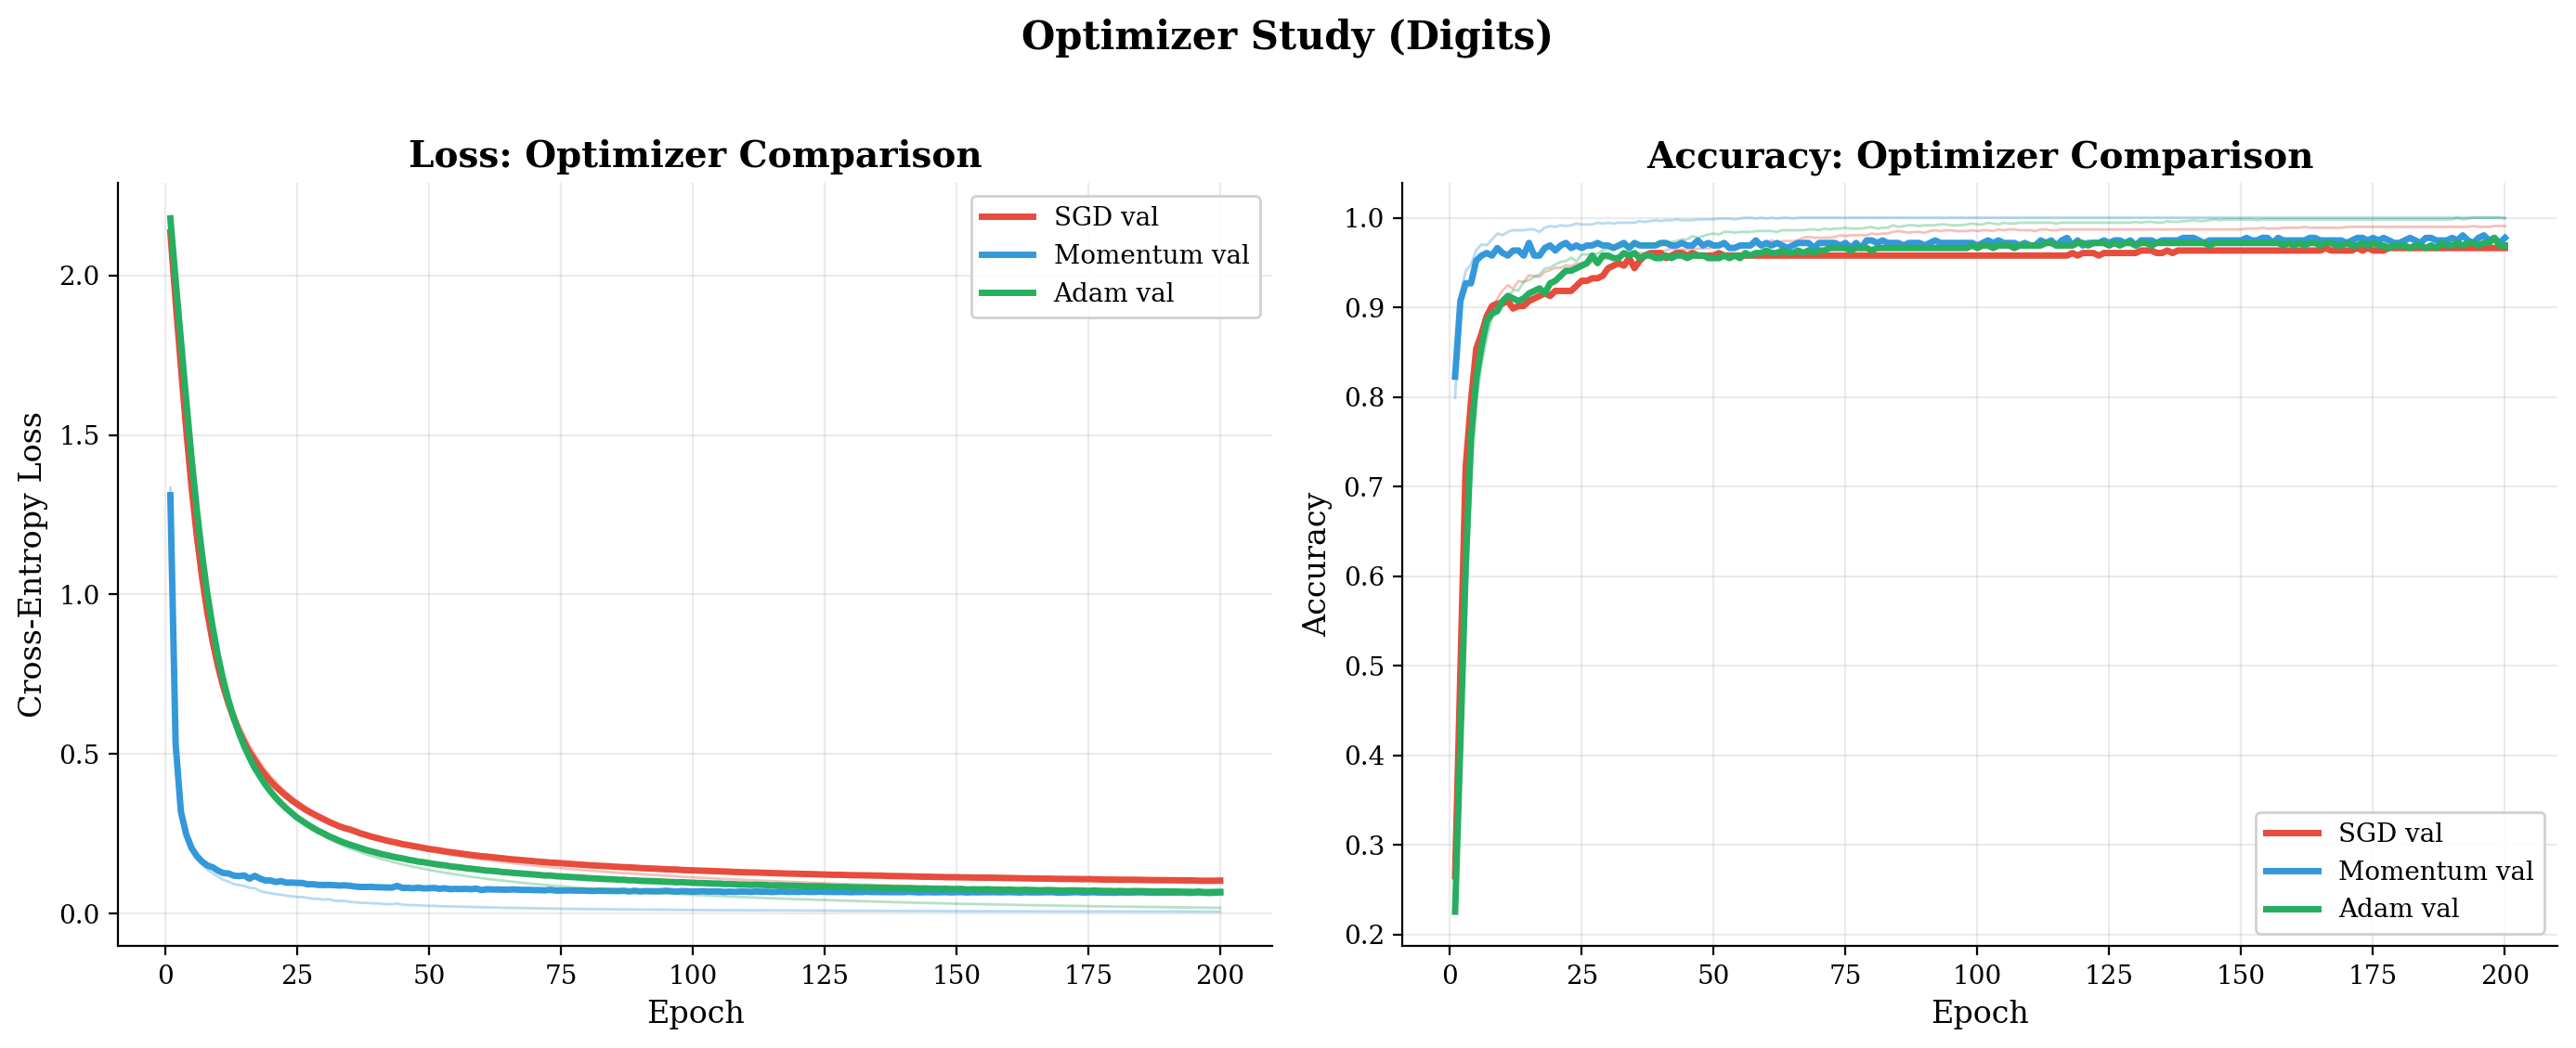
\includegraphics[width=\textwidth]{../figures/optimizer_study_digits.png}
  \caption{Validation loss and accuracy across optimisers (NN, $H{=}32$, Digits).
           Adam and Momentum converge faster; all three reach comparable final performance.}
  \label{fig:optimizers}
\end{figure}

% ──────────────────────────────────────────────────────────────────
\subsection{Failure-Case Analysis: Under-Capacity Bottleneck ($H{=}2$)}
\label{sec:failure}

We deliberately trained a neural network with $H{=}2$ on the 10-class Digits task.  The
hidden layer projects the 64-dimensional input to a 2-dimensional representation via
$\bh = \tanh(\bW_1\bx + \bb_1) \in [-1,1]^2$ before the output layer attempts to
classify into 10~classes.

\begin{table}[H]
\centering
\caption{Failure case: $H{=}2$ bottleneck on Digits.}
\label{tab:failure}
\begin{tabular}{@{}lcc@{}}
\toprule
\textbf{Model} & \textbf{Test Accuracy} & \textbf{Test Cross-Entropy} \\
\midrule
Softmax Regression (linear) & 93.26\% & 0.2692 \\
NN ($H{=}2$) & 58.97\% & 1.1133 \\
NN ($H{=}32$) & 95.71\% & 0.1566 \\
\bottomrule
\end{tabular}
\end{table}

The $H{=}2$ model achieves only $58.97\%$ accuracy---far below even the linear baseline
($93.26\%$).  This is a striking result: a nonlinear model with a hidden layer performs
\emph{worse} than a linear model without one.

\paragraph{Why it fails: a geometric argument.}
The failure is \emph{representational}, not optimisational.  With $H{=}2$, the hidden
layer maps $\R^{64}$ to $[-1,1]^2$.  The output layer then has access to only a
2-dimensional input from which it must carve out 10 linearly separable regions.  In
$\R^2$, the maximum number of regions that $K$ hyperplanes can create is
$\binom{K}{0}+\binom{K}{1}+\binom{K}{2}$, but separating 10 classes into distinct convex
regions with only 2-D linear boundaries is geometrically impossible unless the hidden
representation arranges all 10 classes into perfectly separable clusters---which two
coordinates cannot achieve for the complexity of handwritten digits.

The optimiser faithfully minimises the loss \emph{within} the representational constraints
of the architecture, but the global minimum of the $H{=}2$ loss surface itself corresponds
to a poor classifier.  Despite using the same optimiser, learning rate, epoch budget, and
regularisation that yield $95.71\%$ with $H{=}32$, the bottleneck architecture stalls at
$58.97\%$.  Both training and validation loss remain high throughout (Figure~\ref{fig:failure}).

\paragraph{The lesson.}
\textbf{Representational capacity must match task complexity before optimisation can be
effective.}  Increasing $H$ from 2 to 32 does not change the optimiser---it changes the
\emph{geometry of the function class}, enabling richer internal representations.  This
failure case also explains why adding a hidden layer is not inherently beneficial: if the
width is insufficient, the bottleneck can actually \emph{destroy} information present in
the original input, making the nonlinear model worse than the linear baseline that
preserves all $d$ dimensions.

\begin{figure}[H]
  \centering
  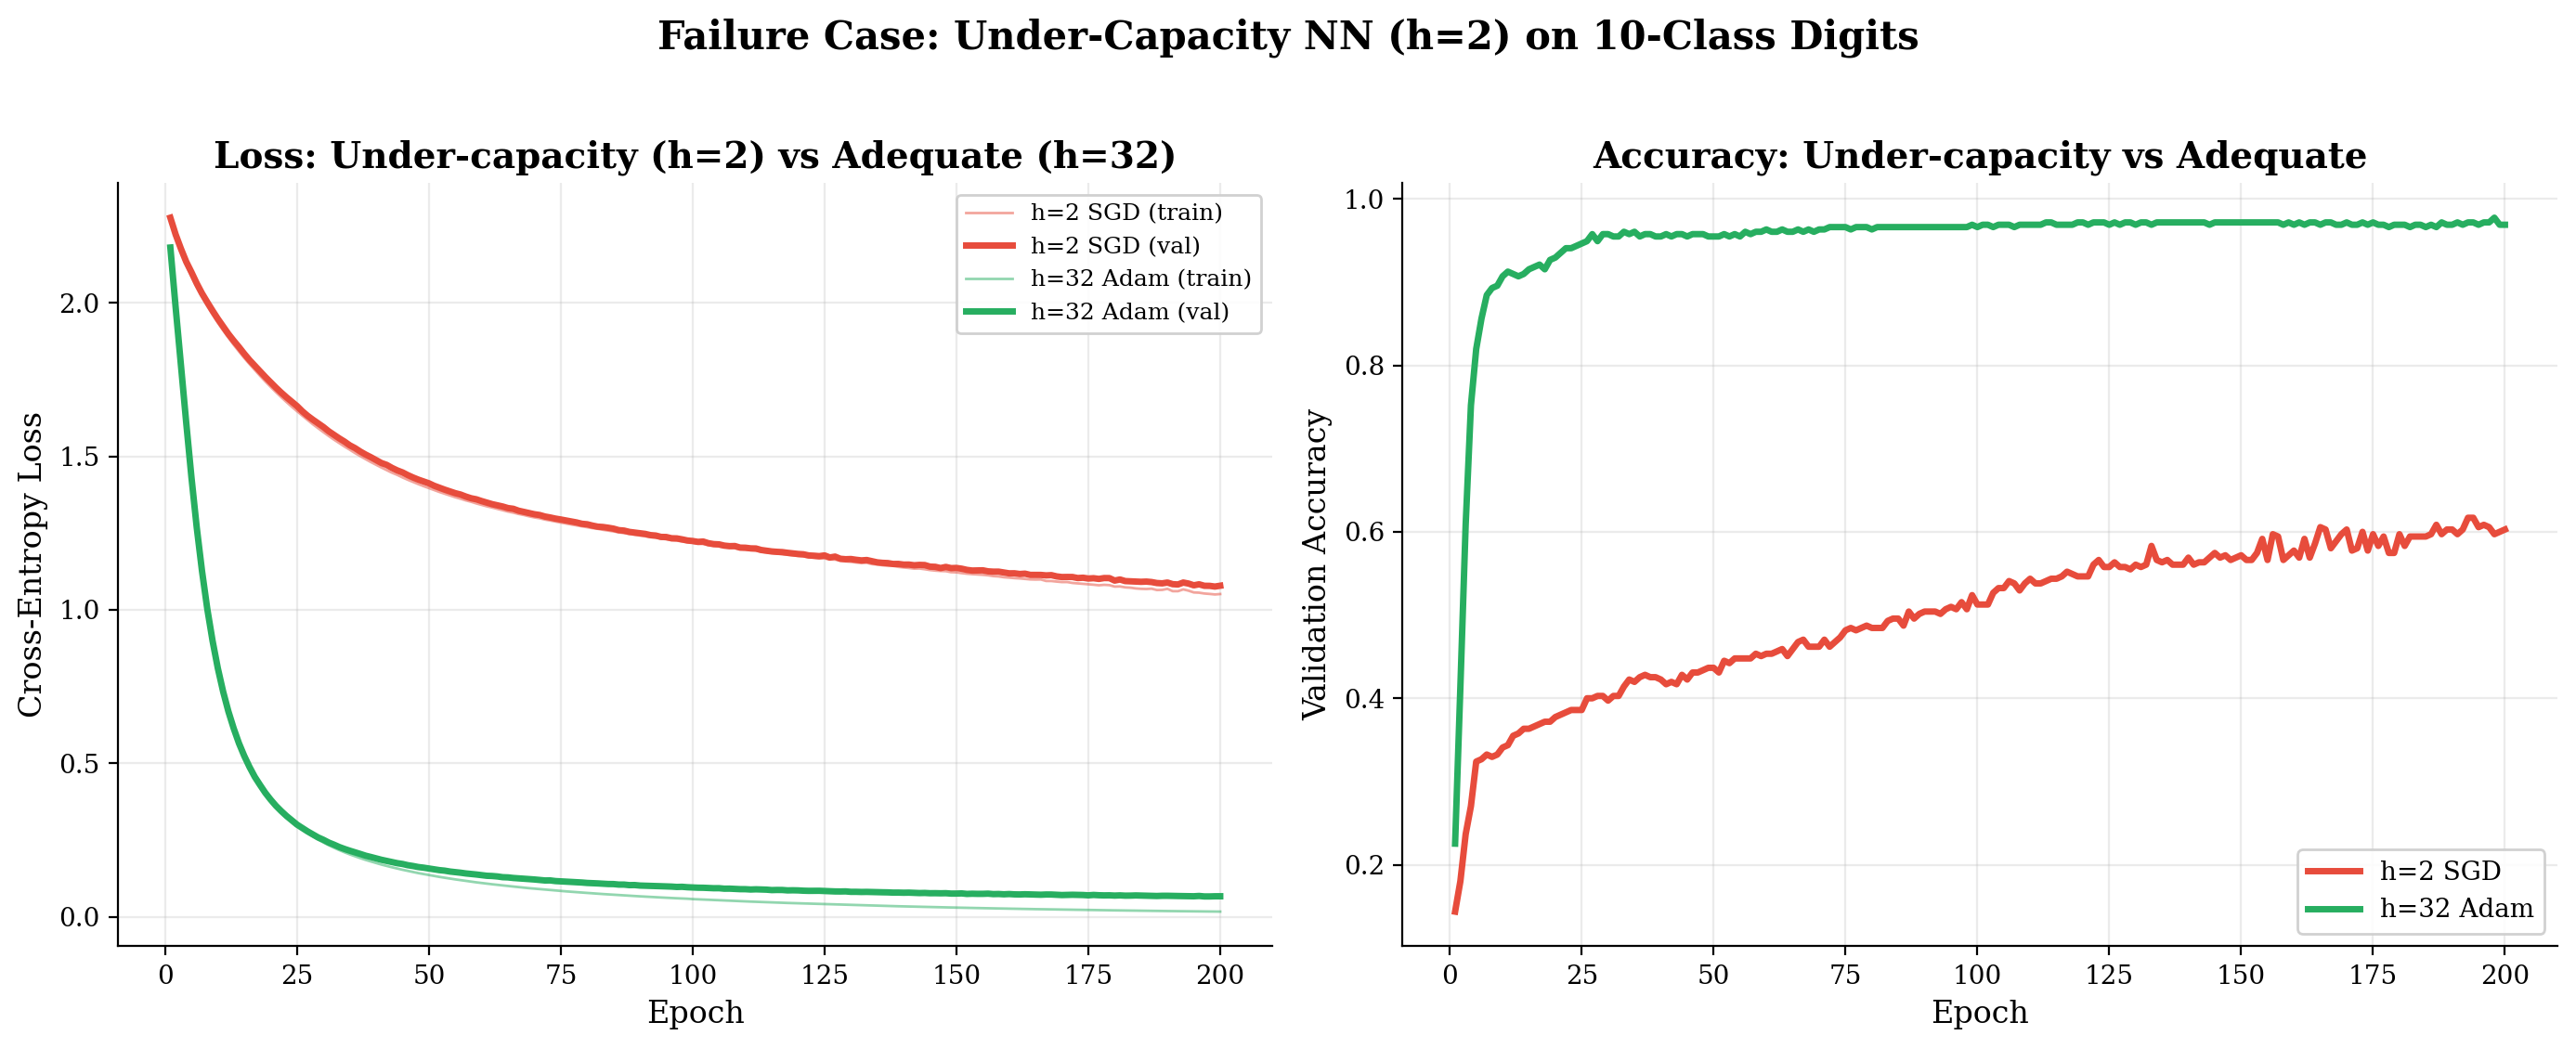
\includegraphics[width=\textwidth]{../figures/failure_analysis.png}
  \caption{Failure case.  The $H{=}2$ bottleneck (red) severely underfits with high
           residual loss, while the $H{=}32$ model (green) converges to low loss.  The
           gap is due to representational capacity, not optimisation quality.}
  \label{fig:failure}
\end{figure}

% ================================================================
\section{Advanced Track A: PCA/SVD and Input Geometry}
\label{sec:pca}
% ================================================================

To study the linear structure already present in the Digits input space before any learning
occurs, we computed the singular value decomposition (SVD) of the mean-centred training
matrix: $\bX_c = \bX - \bone\bar{\bx}^\top$, giving $\bX_c = \mathbf{U}\mathbf{\Sigma}\mathbf{V}^\top$.
The columns of $\mathbf{V}$ are the principal directions; the diagonal entries of
$\mathbf{\Sigma}$ measure the standard deviation of the data along each direction.

\paragraph{Scree analysis.}
Figure~\ref{fig:pca_scree} plots the individual and cumulative explained variance ratios.
The singular values decay rapidly:

\begin{center}
\begin{tabular}{@{}lcccc@{}}
\toprule
Components $m$ & 5 & 10 & 20 & 40 \\
\midrule
Cumulative variance & 54.7\% & 74.1\% & 89.6\% & 98.9\% \\
\bottomrule
\end{tabular}
\end{center}

\noindent
The top 20 components capture $89.6\%$ of total variance; the remaining 44~dimensions
contribute noise-level variance.  This rapid decay indicates that the $8{\times}8$
pixel space has substantial low-dimensional structure---most of the meaningful variation
in digit images lives in a subspace of dimension ${\sim}20$.

\paragraph{2-D projection.}
Figure~\ref{fig:pca_2d} shows the full dataset projected onto the first two principal
components.  Several observations emerge:
\begin{itemize}[leftmargin=1.4em,itemsep=0.15em]
  \item Digits 0 and 6 form relatively distinct clusters, suggesting that their dominant
        pixel patterns differ substantially from other digits.
  \item Digits 3, 5, and 8 overlap heavily, reflecting their visual similarity
        (shared curved strokes).
  \item Two dimensions are insufficient for full 10-class separation, but they reveal
        meaningful coarse structure.
\end{itemize}

\paragraph{Classification at reduced dimensions.}
Table~\ref{tab:pca} reports Softmax Regression validation accuracy when the input is
PCA-compressed to $m$ dimensions:

\begin{table}[H]
\centering
\caption{Softmax Regression accuracy on PCA-reduced Digits inputs.}
\label{tab:pca}
\begin{tabular}{@{}lcccc@{}}
\toprule
$m$ & 10 & 20 & 40 & 64 (full) \\
\midrule
Val.\ Accuracy & 92.68\% & 94.08\% & 94.93\% & 95.49\% \\
Val.\ CE Loss  & 0.2874  & 0.2292  & 0.2133  & 0.2109  \\
\bottomrule
\end{tabular}
\end{table}

At $m{=}20$ (capturing $89.6\%$ of variance), Softmax Regression still achieves
$94.08\%$---only $1.4$ points below the full-dimensional linear result.  This reveals
that \textbf{the Digits input space contains substantial linear structure}: a linear
model can classify well even after discarding $68.75\%$ of the original dimensions.

\paragraph{Connecting back to the main question.}
The PCA experiment places the neural network's ${\sim}2.5$-point advantage in context.
If a linear model on 20 principal components already reaches $94.08\%$, the nonlinear
features captured by the hidden layer exploit only the \emph{residual} $10.4\%$ of
variance plus any \emph{nonlinear} interactions that PCA---a strictly linear
projection---cannot recover.  The hidden layer's value on Digits is real but modest,
consistent with a dataset that is ``mostly linear'' in its discriminative structure.

\begin{figure}[H]
  \centering
  \begin{subfigure}[b]{0.48\textwidth}
    \centering
    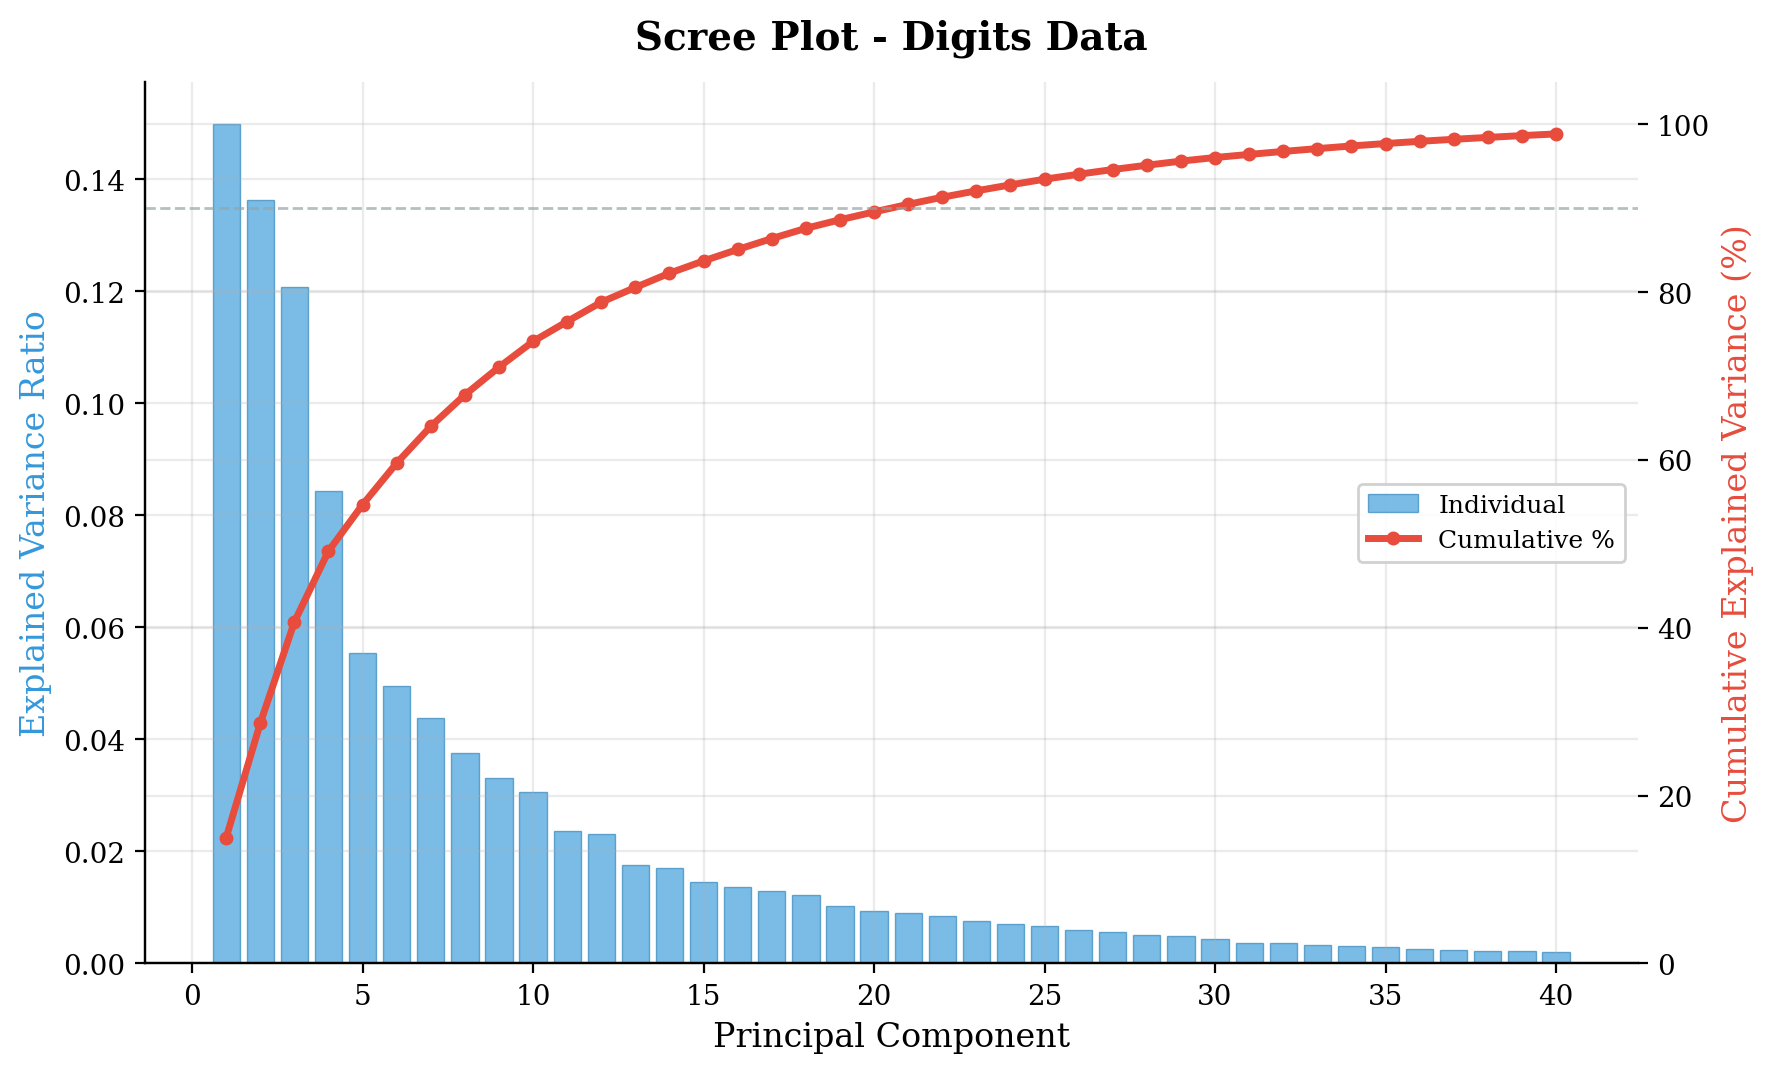
\includegraphics[width=\textwidth]{../figures/pca_scree_digits.png}
    \caption{Scree plot and cumulative explained variance.}
    \label{fig:pca_scree}
  \end{subfigure}\hfill
  \begin{subfigure}[b]{0.48\textwidth}
    \centering
    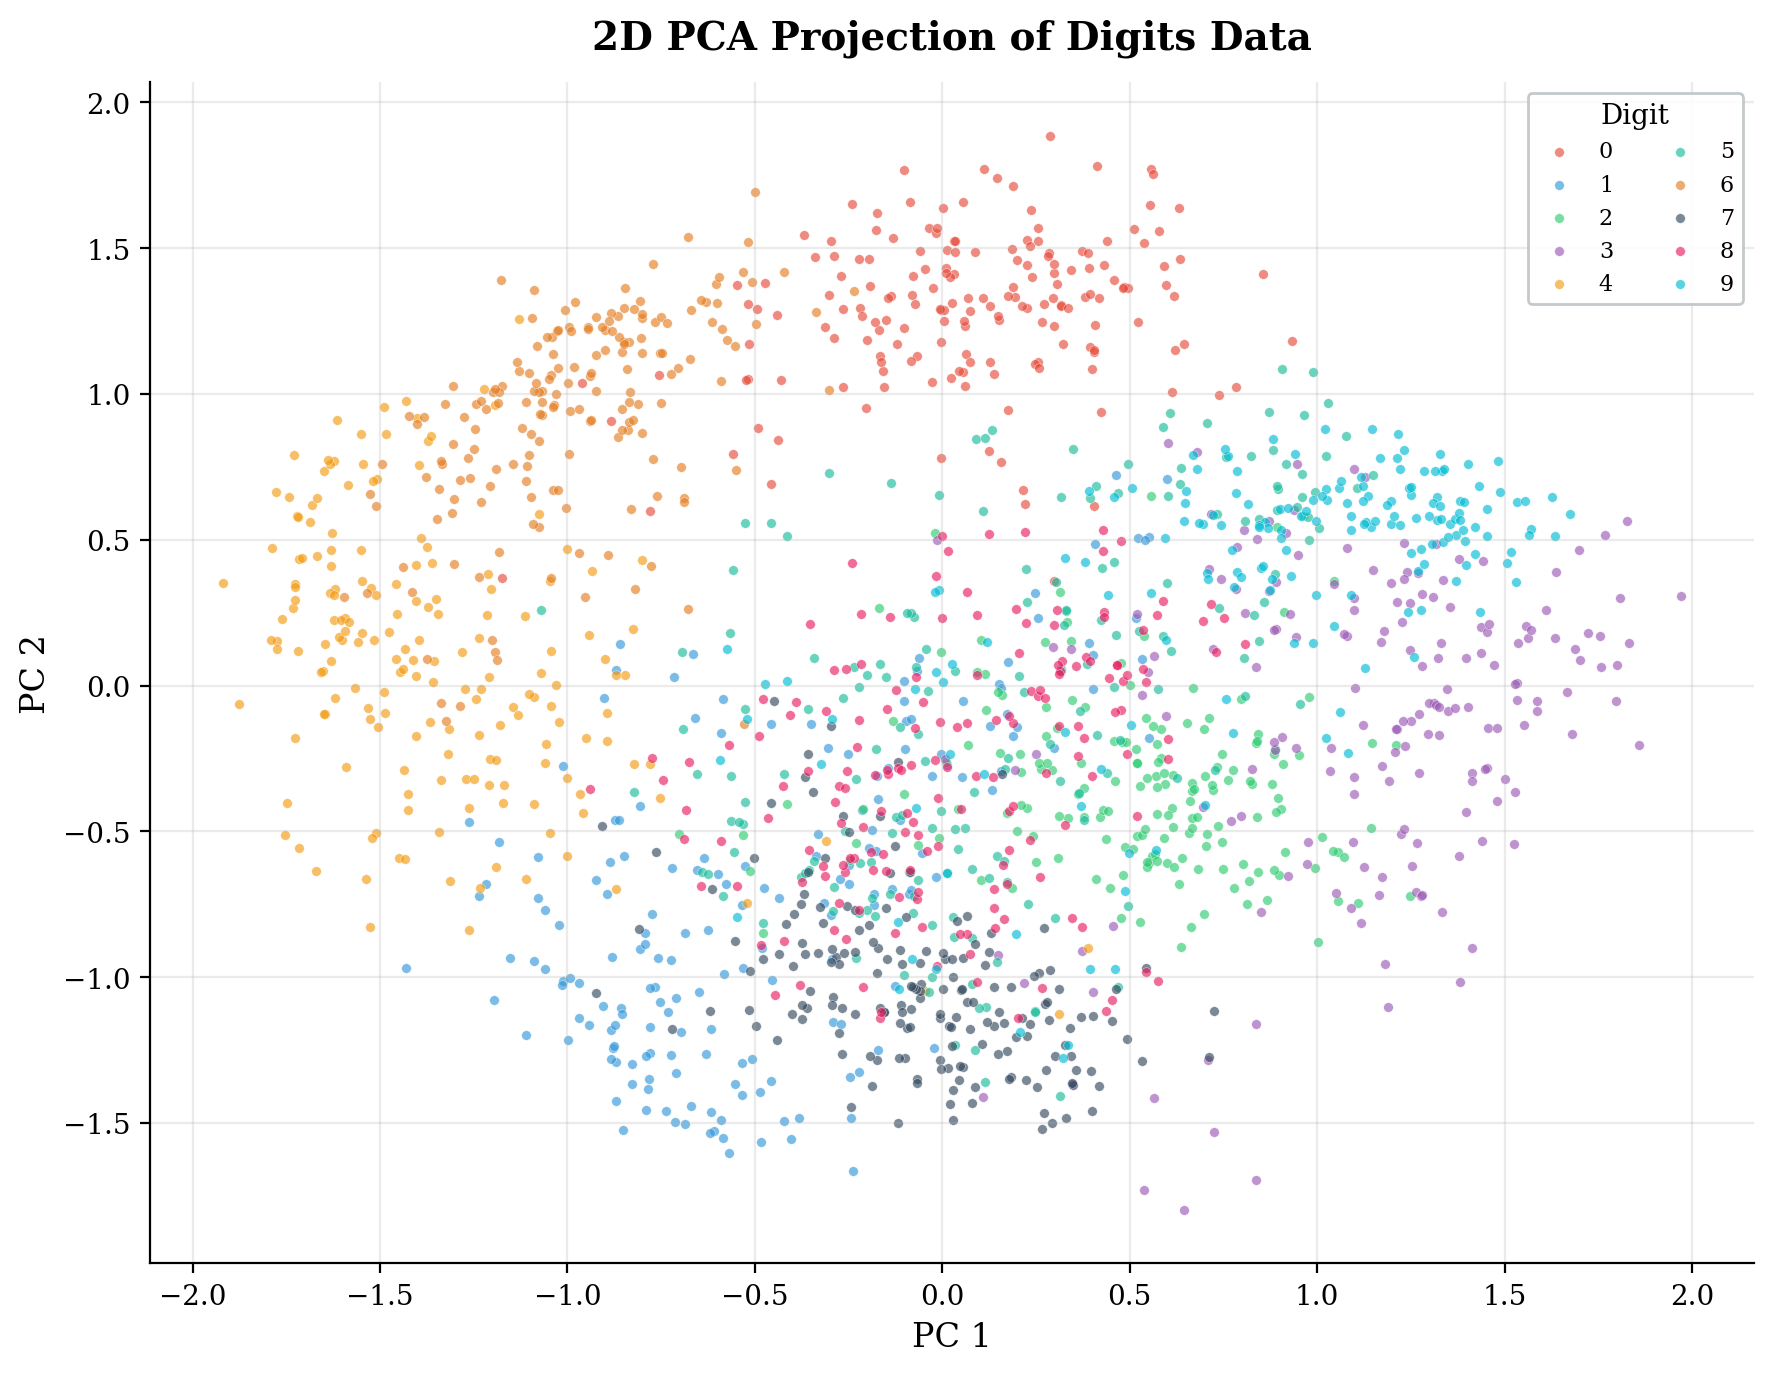
\includegraphics[width=\textwidth]{../figures/pca_2d_digits.png}
    \caption{2-D PCA projection of Digits classes.}
    \label{fig:pca_2d}
  \end{subfigure}
  \caption{Track A: PCA/SVD analysis of the Digits dataset.  The rapid variance decay
           (left) and partial cluster separation (right) reveal substantial linear
           structure.}
  \label{fig:pca}
\end{figure}

% ================================================================
\section{Discussion: Interpretive Analysis}
\label{sec:discussion}
% ================================================================

We now answer the five core interpretive questions, drawing exclusively on the mathematical
framework and experimental evidence developed in this report.

\begin{enumerate}[leftmargin=2em,itemsep=0.6em]

\item \textbf{When is the linear model geometrically sufficient, and when is it not?}

The linear model is sufficient whenever the class-conditional distributions produce a
Bayes-optimal boundary that is a hyperplane (or close to one).  This is rigorously the
case for the Linear Gaussian task: Equation~\eqref{eq:logodds} shows that the log-odds
are affine in~$\bx$, so Softmax Regression can represent the optimal classifier exactly.
It is approximately true for Digits, where Softmax Regression achieves $93.26\%$
and the PCA experiment (Table~\ref{tab:pca}) confirms that the dominant discriminative
directions are linear.

The linear model is \emph{insufficient} when the support regions of the classes create
boundaries that must curve.  On Moons, no affine function can separate the two arcs
(Figure~\ref{fig:comparison_moons}), and Softmax Regression produces a qualitatively
incorrect boundary.

\item \textbf{What representational change does the hidden layer provide in your experiments?}

The hidden layer applies $\bh = \tanh(\bW_1\bx+\bb_1)$, a learned nonlinear coordinate
change from $\R^d$ to $\R^H$.  On Moons, this transformation ``untwists'' the
interleaving arcs: points from the two classes that overlap in every linear projection of
$\R^2$ are pulled apart in $\R^{32}$, where the output layer can separate them with a
hyperplane.

On Digits, the transformation captures nonlinear feature combinations---stroke curvatures,
T-junctions, loop closures---that no linear projection can express.  This accounts for the
${\sim}2.5$-point accuracy improvement over Softmax Regression.  The PCA comparison
(Section~\ref{sec:pca}) confirms that this gain comes from \emph{nonlinear} structure:
a linear projection to 20 dimensions already recovers most of the linear discriminative
information, yet the neural network still exceeds it.

\item \textbf{When does additional model complexity fail to justify itself?}

Complexity fails to justify itself in two regimes observed in our experiments:

\emph{(a) When the baseline already captures the essential geometry.}  On the Gaussian
task, the neural network achieves the same accuracy as Softmax Regression with $3.7{\times}$
more parameters.  The additional parameters parameterise $\tanh$ curves that collapse to
near-linear behaviour because the data does not reward nonlinearity.

\emph{(b) When the added complexity is of the wrong kind.}  On Digits, Softmax Regression
at $m{=}20$ PCA dimensions achieves $94.08\%$, within $1.6$ points of the full neural
network ($95.71\%$), using a far simpler pipeline.  If the engineering cost of maintaining
a neural-network implementation is high and a 1.6-point accuracy difference is tolerable,
the linear model on reduced dimensions may be the better practical choice.

\item \textbf{What does your failure case teach about optimisation, capacity, or
generalisation?}

The $H{=}2$ bottleneck experiment (Section~\ref{sec:failure}) teaches that
\emph{representational capacity is a prerequisite that optimisation cannot substitute}.
Despite identical optimiser settings, the $H{=}2$ model stalls at $58.97\%$---below even
the linear baseline.  The bottleneck destroys the 64-dimensional input structure by
compressing it to 2~dimensions, and no amount of gradient descent can recover information
that the architecture discards.

This distinguishes three failure modes:
\begin{itemize}[leftmargin=1.4em,itemsep=0.1em]
  \item \emph{Optimisation failure}: the architecture can represent a good solution, but
        the optimiser cannot find it (e.g.\ bad learning rate, too few epochs).
  \item \emph{Capacity failure}: the architecture \emph{cannot} represent a good
        solution regardless of optimiser quality.  This is what $H{=}2$ on Digits
        demonstrates.
  \item \emph{Generalisation failure}: the model fits training data well but not test
        data (overfitting).  Neither model exhibits this within our protocol.
\end{itemize}

The $H{=}2$ case is pure capacity failure.  Increasing hidden width from 2 to 32 does not
improve the optimiser; it expands the hypothesis class so that a good solution becomes
representable.

\item \textbf{What do repeated-seed statistics add beyond a single run?}

A single training run's outcome depends on the random initialisation of all weight
matrices and the mini-batch permutation order.  A fortunate seed may initialise near a
favourable basin; an unfortunate one may converge to a worse local minimum.  By running
five seeds and reporting $\bar{x}\pm 2.776\cdot s/\!\sqrt{5}$, we bound the
\emph{expected} performance under typical initialisation conditions rather than reporting
a cherry-picked best (or worst) case.

Concretely, the tight intervals (Softmax: $\pm 0.73\%$; NN: $\pm 0.91\%$) confirm that:
\begin{itemize}[leftmargin=1.4em,itemsep=0.1em]
  \item The ${\sim}2.5$-point accuracy gap is robust across random seeds, not an artefact
        of one favourable initialisation.
  \item The neural network has slightly higher variance ($\pm 0.91\%$ vs.\ $\pm 0.73\%$),
        which is expected: more parameters create more sensitivity to initialisation.
  \item Both models are stable enough that practitioner decisions based on these numbers
        are reliable.
\end{itemize}

Without repeated seeds, we could not distinguish a genuine model-class advantage from
random variation.

\end{enumerate}

% ================================================================
\section{Limitations}
\label{sec:limitations}
% ================================================================

Several boundaries constrain the conclusions of this study, and they should be stated
explicitly to prevent overgeneralisation:

\begin{enumerate}[leftmargin=2em,itemsep=0.3em]
  \item \textbf{Architectural scope.}
        We test only a single hidden layer with $\tanh$ activations and widths up to
        $H{=}32$.  Our conclusions about when nonlinearity helps do not extend to deeper
        networks, wider layers, or other activation functions (e.g.\ ReLU, GELU, Swish).
        Deeper architectures can learn hierarchical features that a single hidden layer
        cannot, and our study says nothing about that regime.

  \item \textbf{Dataset scale and diversity.}
        The Digits benchmark has $d{=}64$, $K{=}10$, and ${\sim}1{,}800$ total samples.
        These are toy-scale dimensions by modern standards.  Results may not generalise to
        high-resolution images (e.g.\ CIFAR-10, ImageNet), natural-language data, or tasks
        with hundreds or thousands of classes where the relative advantage of nonlinearity
        may be much larger.

  \item \textbf{Optimiser exploration.}
        Each optimiser is tested with a single fixed hyperparameter setting as specified by
        the protocol.  We cannot claim that SGD is fundamentally inferior to Adam; a
        different learning rate schedule, warm-up period, or gradient clipping strategy
        could change the ranking.  The optimiser comparison reflects \emph{these specific
        settings}, not the optimiser families in general.

  \item \textbf{Regularisation.}
        We use only $L_2$ regularisation ($\lambda{=}10^{-4}$).  Techniques such as
        dropout, batch normalisation, data augmentation, or learning-rate scheduling might
        change the relative advantage of the neural network on Digits.  Our study does not
        test whether the neural network's gains would increase or decrease under more
        sophisticated training pipelines.

  \item \textbf{Repeated-seed sample size.}
        Five seeds provide a coarse estimate of variability.  The $t$-based confidence
        intervals assume approximate normality of the sample mean; with only five
        observations, this assumption is difficult to verify rigorously.  A larger number
        of seeds (e.g.\ 30) would produce tighter, more reliable intervals.

  \item \textbf{Synthetic task simplicity.}
        The Gaussian and Moons datasets are 2-D with 400~points and noise-free class
        labels.  They illustrate geometric principles clearly but do not represent the
        ambiguity, noise, and high dimensionality of real-world classification tasks.

  \item \textbf{Single data split.}
        All test-set evaluations use a single fixed split.  A more robust assessment would
        employ cross-validation or multiple independent splits, which was outside the scope
        of this project.

  \item \textbf{No calibration analysis.}
        While cross-entropy reduction suggests better probability calibration for the neural
        network, we did not perform formal calibration analysis (e.g.\ reliability diagrams,
        expected calibration error).  Claims about calibration remain informal.
\end{enumerate}

In summary, our findings reliably characterise the specific comparison between Softmax
Regression and a minimal one-hidden-layer network on the three provided tasks under the
fixed protocol.  They should not be overgeneralised to deeper architectures, larger
datasets, different activation functions, or more sophisticated training pipelines.

% ================================================================
\newpage
\section*{References}
% ================================================================
\begin{enumerate}[label={[\arabic*]},leftmargin=2em,itemsep=0.2em]
  \item Deisenroth,~M.\,P., Faisal,~A.\,A., \& Ong,~C.\,S.\ (2020). \textit{Mathematics
        for Machine Learning}. Cambridge University Press.
  \item Murphy,~K.\,P.\ (2022). \textit{Probabilistic Machine Learning: An Introduction}.
        MIT Press.
  \item Goodfellow,~I., Bengio,~Y., \& Courville,~A.\ (2016). \textit{Deep Learning}. MIT
        Press.
  \item Ng,~A.\ \& Katanforoosh,~K. \textit{CS229 Lecture Notes: Deep Learning}. Stanford
        University.  Available at \url{https://cs229.stanford.edu/}.
  \item Stanford CS231n staff. \textit{Neural Networks Part 1: Setting up the Architecture}.
        \url{https://cs231n.github.io/neural-networks-1/}
  \item Stanford CS231n staff. \textit{Optimization Part 2: Backpropagation, Intuitions}.
        \url{https://cs231n.github.io/optimization-2/}
  \item ETH Zurich Learning and Adaptive Systems Group. \textit{Introduction to Machine
        Learning Course Notes}.
        \url{https://las.inf.ethz.ch/teaching/introml-s24}
  \item GitHub. \textit{GitHub Flow}.
        \url{https://docs.github.com/en/get-started/using-github/github-flow}
  \item MIT CSAIL. \textit{The Missing Semester of Your CS Education: Version Control (Git)}.
        \url{https://missing.csail.mit.edu/2020/version-control/}
  \item Math4AI Program Handout: \textit{Math4AI Capstone: From Linear Scores to a Single
        Hidden Layer}. National AI Center --- AI Academy, 2026.
\end{enumerate}

\end{document}
